% Preamble
\documentclass[12pt]{CLASS/protokol}
% --------


% Definice proměnných pro titulní stránku
% Přepište text v složených závorkách na požadované hodnoty
% např: {Datum měření} -> {1.1.1900}
\newcommand{\predmet}{Modelování a počítačová simulace}
\newcommand{\uloha}{Zdroj proudu s~vhodnou napěťovou referencí}
\newcommand{\jmeno}{Lukáš Lev, 256660}
% -------------------------------------

%-----Bibliografie-----
\usepackage[backend=biber,style=numeric,citestyle=numeric,sorting=none,language=czech]{biblatex}
\DefineBibliographyStrings{czech}{
  references = {Seznam použité literatury}, % Nastaví jméno referencí
}

\addbibresource{citace.bib} % Soubor s citacemi v BibLaTeXu

% Pouzite balicky
\usepackage{comment}
\usepackage{fancyhdr} % For custom headers and footers
\usepackage{graphicx}
\usepackage{listings}
\usepackage{xcolor}
\usepackage{subcaption}

% listing
\renewcommand{\lstlistingname}{Úryvek kódu}
\renewcommand{\lstlistlistingname}{Seznam úryvků kódu}

% Define a color scheme
\definecolor{codebg}{RGB}{248,248,255} % very light gray-blue
\definecolor{codeframe}{RGB}{100,100,120} % darker gray-blue
\definecolor{keywordcolor}{RGB}{0,0,180} % strong blue
\definecolor{commentcolor}{RGB}{0,128,0} % green
\definecolor{stringcolor}{RGB}{163,21,21} % dark red

% Set font
\usepackage{courier} % or choose another font you like
\renewcommand{\ttdefault}{pcr} % Courier

% Define the listings style
\lstdefinestyle{mystyle}{
    backgroundcolor=\color{codebg},
    frame=single,
    rulecolor=\color{codeframe},
    basicstyle=\ttfamily\small, % font type and size
    keywordstyle=\color{keywordcolor}\bfseries,
    commentstyle=\color{commentcolor}\itshape,
    stringstyle=\color{stringcolor},
    numbers=left,
    numberstyle=\tiny\color{gray},
    numbersep=8pt,
    tabsize=4,
    breaklines=true,
    showstringspaces=false,
    captionpos=b
}

% Apply the style globally
\lstset{style=mystyle}



% Document
\begin{document}            % document start
\pagenumbering{gobble}      % číslování stránek
\pagenumbering{arabic}      % číslování stránek
\pagestyle{empty}           % bez číslování
%%%%%%%%%%%%%%%%%%%%%%%%%%%%%%%%%%%%%%%%%%%%%%%%%%%%%%%%%
%														%
%     Tuto Šablonu vytvořil Ing. Pavel Čudek, Ph.D.     %
%			pro potřeby předmětů DME a DIZ 				%
%														%
%%%%%%%%%%%%%%%%%%%%%%%%%%%%%%%%%%%%%%%%%%%%%%%%%%%%%%%%%
%                                                       %
% Tento soubor slouží ke generování titulní strany      %
% samostatné práce. Nic v tomto dokumentu neměňte.      %
% Titulnístrana se generuje automaticky z hodnot        %
% zadaných v souboru SP_Text.tex                        %
%                                                       %
%%%%%%%%%%%%%%%%%%%%%%%%%%%%%%%%%%%%%%%%%%%%%%%%%%%%%%%%%

\begin{titlepage}
	\begin{tikzpicture}[remember picture, overlay]
		\draw[line width = 2pt] ($(current page.north west) + (1cm,-1cm)$) rectangle ($(current page.south east) + (-1cm,1cm)$);
	\end{tikzpicture}

	\begin{center}
		\vspace{-1.5cm}
        
		\begin{figure}[!h]
            \centering
			
\includegraphics[width=14cm]{obrazky/umel.png}
		\end{figure}

		\vspace{3.5cm}

		{SEMESTRÁLNÍ PRÁCE Z PŘEDMĚTU}\\
		\vspace{0.25cm}

		\large{\textbf{\predmet}}\\
		\vspace{3.5cm}

		\textbf{NÁZEV PRÁCE: \uloha}
		\vspace{2.5cm}\\
		\vfill
    
	\end{center}
        \begin{tabular}{ll}
            semestr: & LS 2024/2025 \\
            skupina: & Út 18:00 \\
            vypracoval: & {\jmeno} \\
            datum: & \today
        \end{tabular}
\end{titlepage}  % Neměnit, odkaz na protokol_title.tex
\clearpage                  %
\setcounter{page}{2}        % Nastavení čísla druhé stránky na 2
\newpage                    % nová stránka (strana 2)

\tableofcontents            % Automaticky generovaný obsah
\newpage
\clearpage\pagestyle{plain} % Zapnout číslování stránek

% header
\pagestyle{fancy}
\fancyhf{} % Clear default header and footer
\fancyhead[R]{\small\textcolor{black!85}{Zdroj proudu s vhodnou napěťovou referencí}} % Left header with the section name
\fancyfoot[c]{-~\thepage~-} % Centered footer with page number
\renewcommand{\headrulewidth}{1pt}
\renewcommand{\footrulewidth}{1pt}

% Odsud dál pište text práce
% ==========================

\newpage
\section{Zadání}\label{sec:zadani}
    \begin{enumerate}[leftmargin=.6cm]
        \item Získejte z~Internetu nebo jiným způsobem model vybrané vhodné klíčové součástky (Nap\_reference) pro~PSpice.
        \item Získejte katalogový list (datasheet) k~vybrané klíčové součástce.
        \item S modelem klíčové součástky sestavte zdroj proudu (zvolte hodnotu Iout mezi~5~mA a~50~mA) podle doporučeného zapojení.
        \item Experiment č.~1: Změřte teplotní koeficient proudu Iout při zátěži 100~$\Omega$ a~Vcc~=~5~V. Zjistěte závislost proudu Iout na~velikosti zátěže. Ověřte výpočtem maximální hodnotu zátěže, kterou ještě může protékat nastavený konstantní proud.
        \item Experiment č.~2: Analyzujte spektrální hustotu šumového výkonu a~proudu zátěží v~kmitočtovém pásmu 1~Hz až~150~kHz. Zjistěte efektivní hodnotu šumového proudu v~tomto~frekvenčním pásmu (a~srovnejte ji~s~velikostí pracovního proudu Iout).
        \item Experiment č.~3: Proveďte další experiment dle vlastního uvážení.
    \end{enumerate}

\clearpage
\newpage
\section{Charakteristika klíčové součástky}\label{sec:char_soucastky}
    Klíčovou součástkou je TL431 vyráběna společností Texas~Instruments. Vlastnosti této komponenty jsou popsány v~technickém listu vydaném firmou Texas~Instruments \cite{TI_TL431_datasheet}.
    \par
    V kapitole \uv{Detailed Description} této dokumentace je uvedeno ekvivalentní schéma obvodu TL431 (viz~obr.~\ref{fig:ekv_schematic}). Pokud uvážíme, že~vnitřní napěťová reference, označena jako~$V_{ref}$, vytváří mezi svými výstupy přesný napěťový rozdíl 2,5~V (typicky 2,495~V, viz~tab.~\ref{tab:max_ratings}), pročež jsou pro hodnoty katodového napětí platí $V_{KA} \in (2,5;37)$~V.

    \begin{figure}[h]
        \centering
        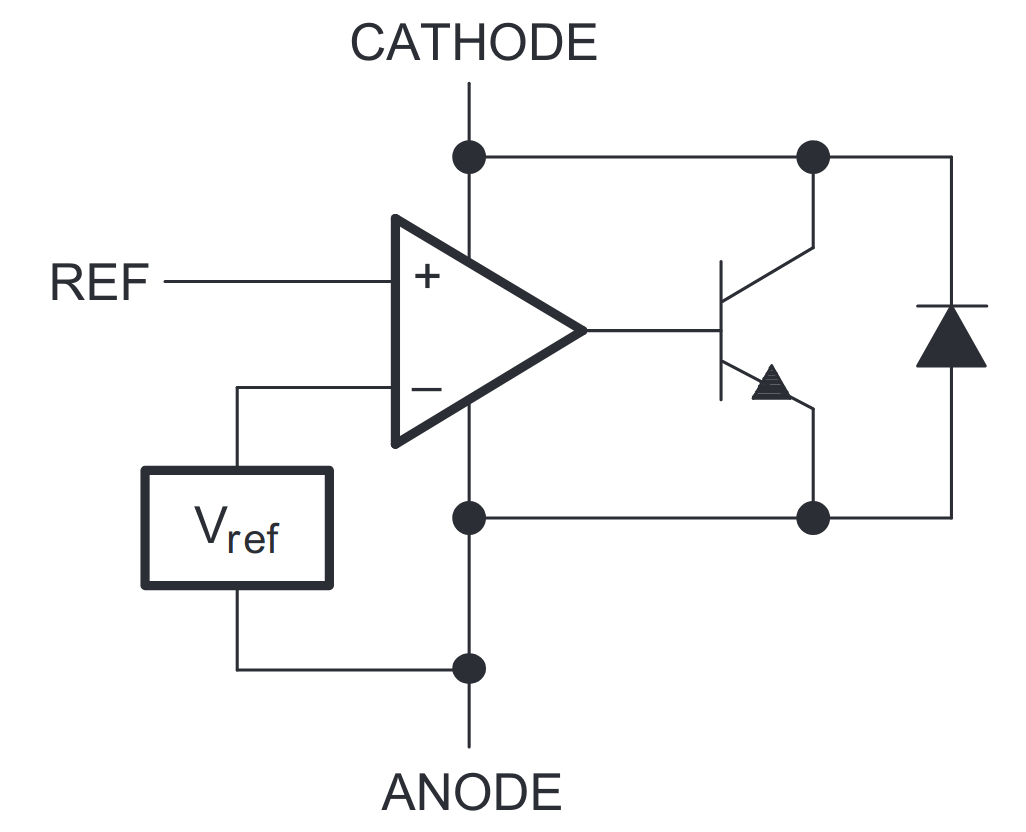
\includegraphics[width=0.5\linewidth]{Sablona_LaTeX/obrazky/ekv_schema.png}
        \caption{Ekvivalentní schéma obvodu TL431\cite{TI_TL431_datasheet}}
        \label{fig:ekv_schematic}
    \end{figure}

    \begin{table}[h]
    \centering
    \caption{Specifikace maximálních operačních parametrů TL431}
    \label{tab:max_ratings}
    \begin{tabular}{rlccc}
    \textbf{}                                   & \textbf{}                  & MIN   & MAX & jednotka  \\ \hline
    \multicolumn{1}{r}{\textbf{$V_{KA}$}}     & katodové napětí            & 2,5   & 37  & V         \\
    \multicolumn{1}{r}{\textbf{$I_{KA}$}}     & kontinuální katodový proud & -100  & 150 & mA        \\
    \multicolumn{1}{r}{\textbf{$I_{I(ref)}$}} & proud referenčním uzlem    & -0,05 & 10  & mA        \\
    \multicolumn{1}{r}{\textbf{$T_J$}}          & pracovní teplotní rozsah   &       & 150 & $^\circ$C \\
    \multicolumn{1}{r}{\textbf{$T_{stg}$}}    & teploty skladování         & -65   & 150 & $^\circ$C
    \end{tabular}
    \end{table}
    
    \par
    Pokud bude tedy na~uzel~REF přivedeno napětí větší než~2,5~V, pak se aktivuje operační zesilovač v~roli komparátoru a~\uv{otevře} bipolární tranzistor, s~jehož bází je spojen. Tranzistor, jímž díky napětí na~bázi teče proud mezi~kolektorem a~emitorem, reguluje napětí v~katodovém uzlu na~2,5~V. V~opačném případě je tranzistor uzavřen a~k~regulaci nedochází.
    \par
    Je nutno poznamenat, že~k~regulačním procesům popsaným výše dochází pouze za~předpokladu dostatečného katodového proudu, jehož minimální hodnota $I_{min}$ je výrobcem stanovena jako 1~mA (viz~tab.~\ref{tab:el_char}).

    \begin{table}[h]
    \centering
    \caption{Specifikace elektrických vlastností TL431 za teploty 25 $^\circ$C}
    \label{tab:el_char}
    \begin{tabular}{llcccc}
    \multicolumn{2}{c}{\textbf{parametr}}              & \multicolumn{1}{l}{\textbf{MIM}} & \multicolumn{1}{l}{\textbf{TYP}} & \multicolumn{1}{l}{\textbf{MAX}} & \multicolumn{1}{l}{\textbf{jednotka}} \\ \hline
    $V_{ref}$ & referenční napětí                     & 2440                             & 2495                             & 2550                             & mV                                    \\
    $I_{ref}$ & vstupní proud reference               &                                  & 2                                & 4                                & $\mu$A                                \\
    $I_{min}$ & minimální katodový proud pro regulaci &                                  & 0,4                              & 1                                & mA                                   
    \end{tabular}
    \end{table}
    
    \par
    Takováto aplikace je popsána také v~dokumentaci výrobce (viz kapitolu Comparator With Integrated Reference). Zároveň bylo toto zapojení ověřeno programem Micro~Cap \cite{Micro_Cap}. Simulované zapojení je na~obr.~\ref{fig:komp_schem} a~výstup tranzientní analýzy v~Micro-Cap je na~obr.~\ref{fig:komp_tran}.

    \begin{figure}[h]
        \centering
        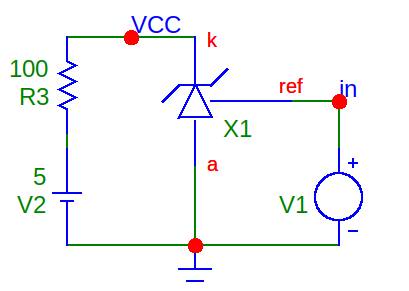
\includegraphics[width=0.5\linewidth]{Sablona_LaTeX/obrazky/komp_schem.png}
        \caption{Zapojení TL431 jako komparátoru s~integrovanou referencí pro~simulaci v~programu Micro-Cap \cite{Micro_Cap}}
        \label{fig:komp_schem}
    \end{figure}

    \begin{figure}[h]
        \centering
        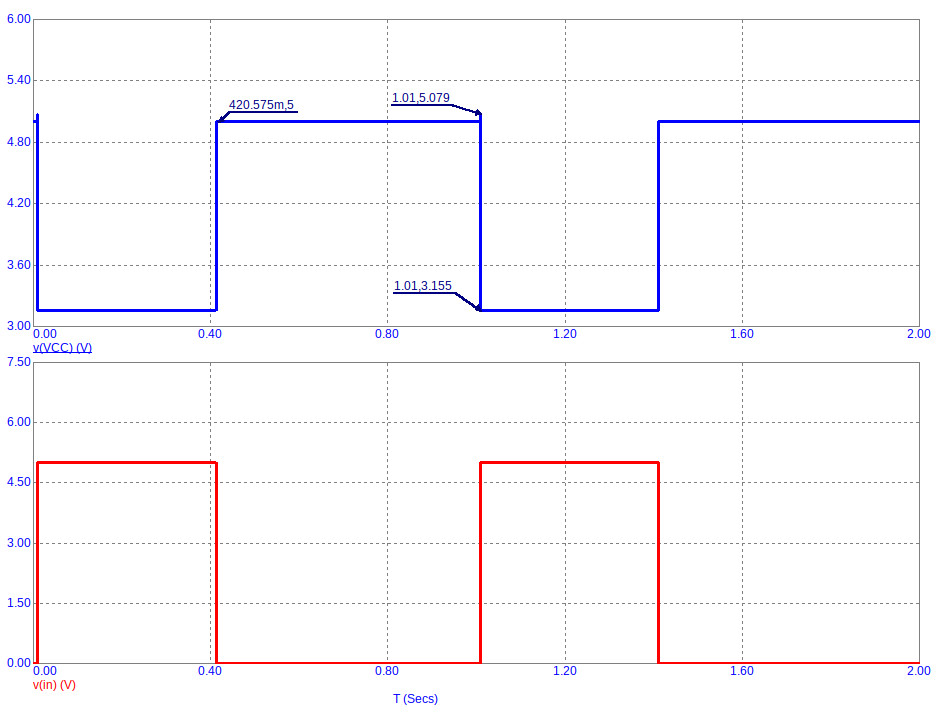
\includegraphics[width=\linewidth]{Sablona_LaTeX/obrazky/komp_signal.jpg}
        \caption{Výstup tranzientní analýzy v~programu Micro-Cap pro zapojení z~obrázku~\ref{fig:komp_schem} \cite{Micro_Cap}}
        \label{fig:komp_tran}
    \end{figure}

    \clearpage
    \par
    Pokud je ve~zpětné vazbě z~uzlu REF zapojen napěťový dělič (viz~obr.~\ref{fig:nastreg_schem}), pak je možno hodnotami odporů $R1$ a~$R2$ nastavit velikost výstupního, regulovaného, napětí $V_O$ podle uvedeného vzorce: $V_O=\left(1+\frac{R1}{R2}\right)V_{ref}$.\cite{TI_TL431_datasheet}

    \begin{figure}[h]
        \centering
        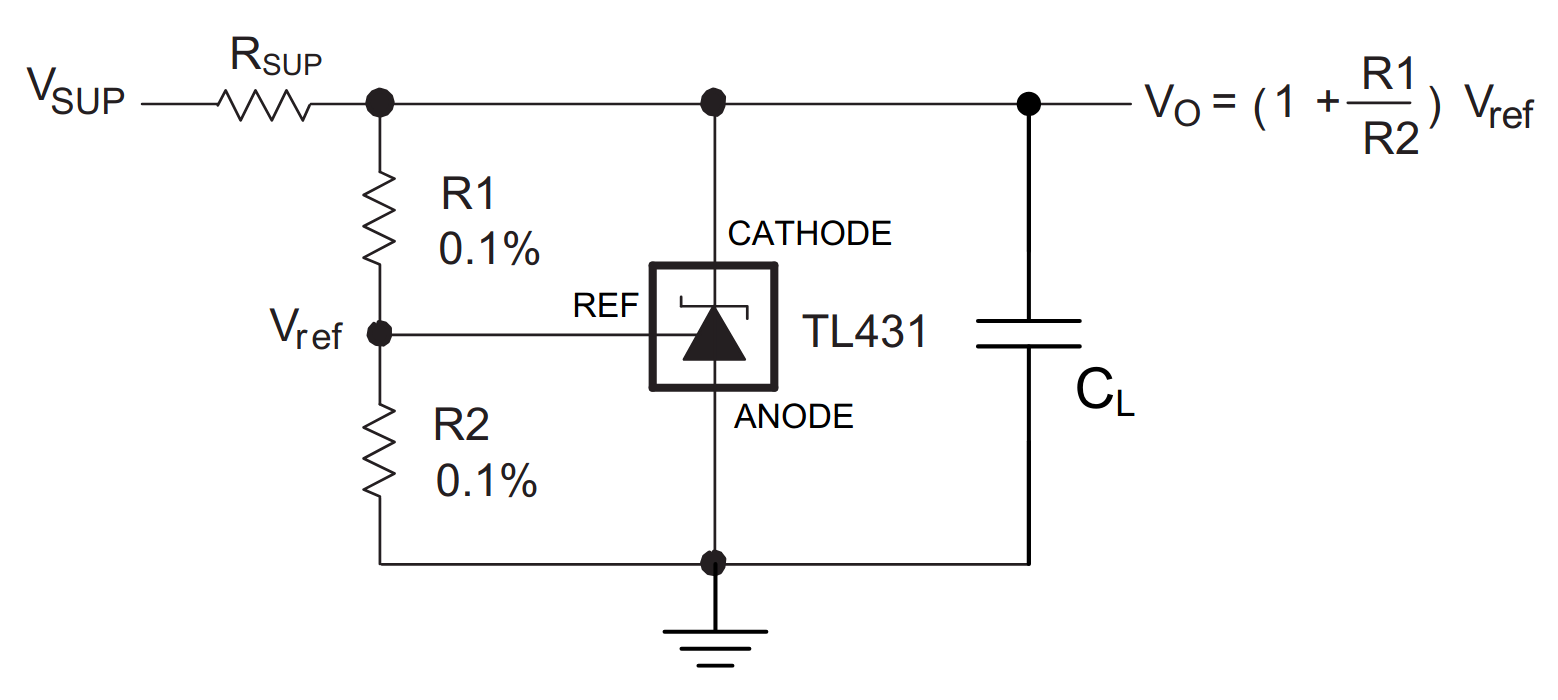
\includegraphics[width=0.75\linewidth]{Sablona_LaTeX/obrazky/nast_reg_schem.png}
        \caption{Nastavitelný regulátor napětí s~využitím TL431 \cite{TI_TL431_datasheet}}
        \label{fig:nastreg_schem}
    \end{figure}
    
    \par
    Dalšími možnými aplikacemi jsou napájecí zdroje, sledovače hladiny napětí, logika ochrany nabíjení a~vybíjení pro~akumulátory a~další \cite{TI_TL431_datasheet}.

    
    
\clearpage
\newpage
\section{Rozhraní modelu klíčové součástky}\label{sec:rozhrani}
    Klíčovou součástkou je TL431 (viz~kapitolu~\ref{sec:char_soucastky}), jež je popsána ve~SPICE modelu TL431.mod. Tento model byl poskytnut společností Texas~Instruments, která jej uvádí na svých internetových stránkách. Podle hlavičky souboru lze stanovit datum vytvoření modelu na~rok~1992 \cite{TL431_spice_model}.
    \par
    Rozhraní modelu sestává ze~tří vývodů (viz~obr.~\ref{fig:TL431_schematic}):
    \begin{enumerate}
        \item reference ---~napětí přivedeno na~tento uzel je srovnáváno s~vnitřní napěťovou referencí~TL431 o~hodnotě 2,5~V,
        \item anoda ---~zápornější elektroda (často spojena se zemí),
        \item katoda ---~kladnější elektroda, jejím výstupem je stabilizované napětí.
    \end{enumerate}
    
    \begin{figure}[h]
        \centering
        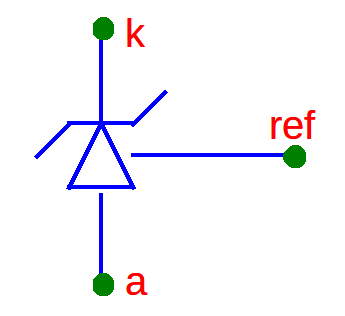
\includegraphics[width=0.25\linewidth]{Sablona_LaTeX/obrazky/TL431_pinout.png}
        \caption{Schematická značka modelu klíčové součástky TL431 s~označenými~vývody}
        \label{fig:TL431_schematic}
    \end{figure}

    \par
    Model je realizován za~zjednodušení operačního zesilovače na~závislý zdroj napětí řízený napětím, jež ovlivňuje velikost proudu tekoucí z~uzlu katody do~anody, a~to~pomocí polynomiální funkce $V(4,anod) \cdot 710 - V(ref,anod) \cdot 710 = V(5,anod)$ (viz~obr.~\ref{fig:model_schem}).
    \par
    Model také zohledňuje teplotní vlivy na~odpor $R2$ a~sériové odpory diod. Lze~ale~předpokládat, že~například při~vysokofrekvenčních aplikacích bude vznikat chyba tohoto modelu v~důsledku nedokonalého modelování vnitřních jevů operačního zesilovače.
    
    \begin{figure}[h]
        \centering
        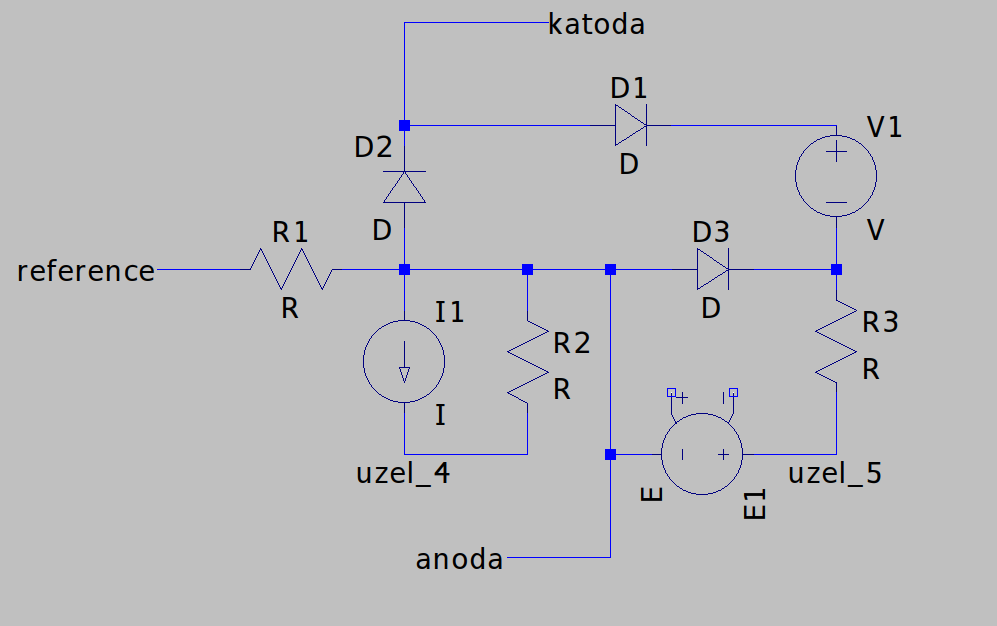
\includegraphics[width=0.7\linewidth]{Sablona_LaTeX/obrazky/SPICE_TL431.png}
        \caption{Zjednodušený model TL431 ve~\uv{SPICE-like} prostředí programu~LTspice~\cite{LTspice}}
        \label{fig:model_schem}
    \end{figure}
    
\clearpage
\newpage
\section{Simulované schéma s~klíčovou součástkou}\label{sec:zapojeni}
    Schéma poskytnuté vyučujícím (obr.~\ref{fig:dop_zap}) odpovídá schématu, jež v~kapitole System Examples uvádí výrobce TL431 pod názvem \uv{Precision Constant-Current Sink} \cite{TI_TL431_datasheet, TI_current_srcs} (obr.~\ref{fig:dop_zap_tex}).
    
    \begin{figure}[h]
        \centering
        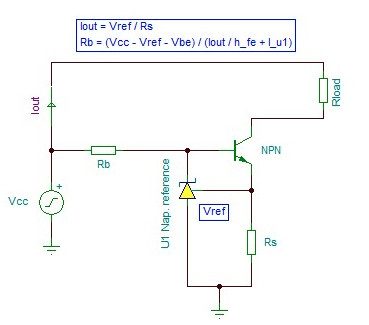
\includegraphics[width=0.5\linewidth]{Sablona_LaTeX/obrazky/dop_zapojeni.jpg}
        \caption{Schéma doporučeného zapojení poskytnutého vyučujícím}
        \label{fig:dop_zap}
    \end{figure}

    \par
    V~tomto zapojení řídí TL431 bázi bipolárního tranzistoru, čímž kontroluje proud ním protékající. Regulace proudu se dosahuje sledováním a~úpravou napětí na~rezistoru $R_s$. Protože veškerý proud zátěže $I_{OUT}$ protéká rezistorem $R_s$, udržování konstantního napětí na $R_s$ zajišťuje konstantní proud zátěží \cite{TI_current_srcs}.
    \par
    Obvod obsahuje rezistor $R_1$ (resp.~$R_b$), který slouží k~nastavení klidového proudu obvodu reference.  Hodnota proudu protékajícího zátěží $I_{OUT}$ je určena vztahem $I_{OUT} = \frac{V_{REF}}{R_S}$.\cite{TI_current_srcs}.

    \begin{figure}[h]
        \centering
        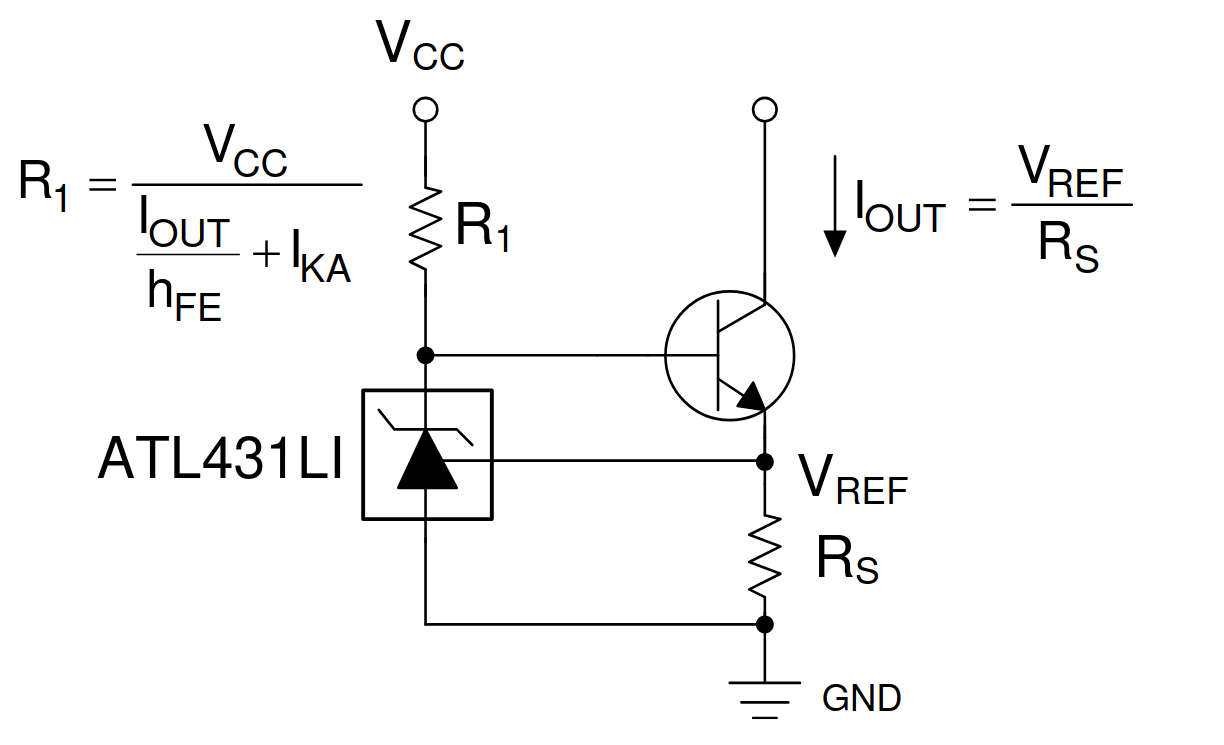
\includegraphics[width=0.65\linewidth]{Sablona_LaTeX/obrazky/dop_zap_texas.png}
        \caption{Schéma doporučeného zapojení poskytnutého výrobcem, kdy může být napěťová reference ATL431LI nahrazena~TL431 \cite{TI_TL431_datasheet, TI_current_srcs}}
        \label{fig:dop_zap_tex}
    \end{figure}
    

    
\clearpage
\newpage
\section{Provedené experimenty}\label{sec:experimenty}
    Výsledky níže popsaných výpočetních experimentů, prováděných pro~zapojení popsané v~kapitole~\ref{sec:zapojeni}, dle zadání poskytnutého vyučujícím (viz~kapitolu~\ref{sec:zadani}), jsou srovnávány s~údaji poskytnutými výrobcem použité součástky TL431 (viz~kapitoly~\ref{sec:char_soucastky} a~\ref{sec:rozhrani}).
    \par
    Všechny simulace byly prováděny v~programech \uv{Spice-like}, tedy vycházejících ze~standardu Spice \cite{spice_berkeley}. Konkrétně byly použity programy LTspice a~PSpice (bližší informace jsou uvedeny v~seznamu použité literatury) \cite{LTspice,student_pspice,pspice}.
    \par
    Tyto programy pro popis zapojení využívají kódové struktury, jež je nazývána netlist. Obecný netlist simulovaného zapojení je uveden v~úryvku kódu~\ref{ls:netlist}. Tato základní struktura byla pro~každý z~experimentů modifikována (především byly nastaveny odpovídající hodnoty součástek).
    \vspace{3.5cm}

    \begin{lstlisting}[label=ls:netlist,caption=Netlist pro zapojení popsané v~kapitole~\ref{sec:zapojeni}]
*** NETLIST ***
Vcc 	in   0         {valVcc}    ;napajeci zdroj
Rb      in   kat       {valRb}     ;odpor pri bazi
Rload   in  col       {valRload}  ;zatez
Rs      ref  0 	       {valRs}     ;odpor pro regulaci
Xref 	ref  0    kat  TL431       ;napetova reference TL431
Q1      col  kat  ref  Q2N2222     ;bipolarni tranzistor pro regulaci

.LIB mps.lib    ;zdrojovy kod soucastky Q1
.LIB tl431.mod  ;zdrojovy kod soucastky Xref
    \end{lstlisting}

    \newpage
    \subsection{Experiment 1a: Teplotní závislost}\label{subsec:1a}
        Aby byl spočten teplotní koeficient $\theta_{Iout}$ byla nastavena hodnota odporu zátěže na~100~$\Omega$ a~napájecí napětí bylo nastaveno na~5~V. Tím bylo zaručeno katodové napětí (v~uzlu kat) větší než 2,5~V, což je podmínka pro regulaci.
        \par
        Pomocí příkazu .step temp, tedy \uv{krokuj teplotu} byl pro jednotlivé výpočty pracovního bodu měněn parametr teploty, za~níž byly parametry simulovány. Z~každého z~dílčích pracovních bodů byla vynesena hodnota proudu součástkou Rload do~závislosti na~obrázku~\ref{fig:1a_i}. Simulace byla provedena v~intervalu stanoveném výrobcem jako pracovní teplotní rozsah (viz~tab.~\ref{tab:max_ratings}).
        \vspace{2cm}
        
        \begin{figure}[h]
            \centering
            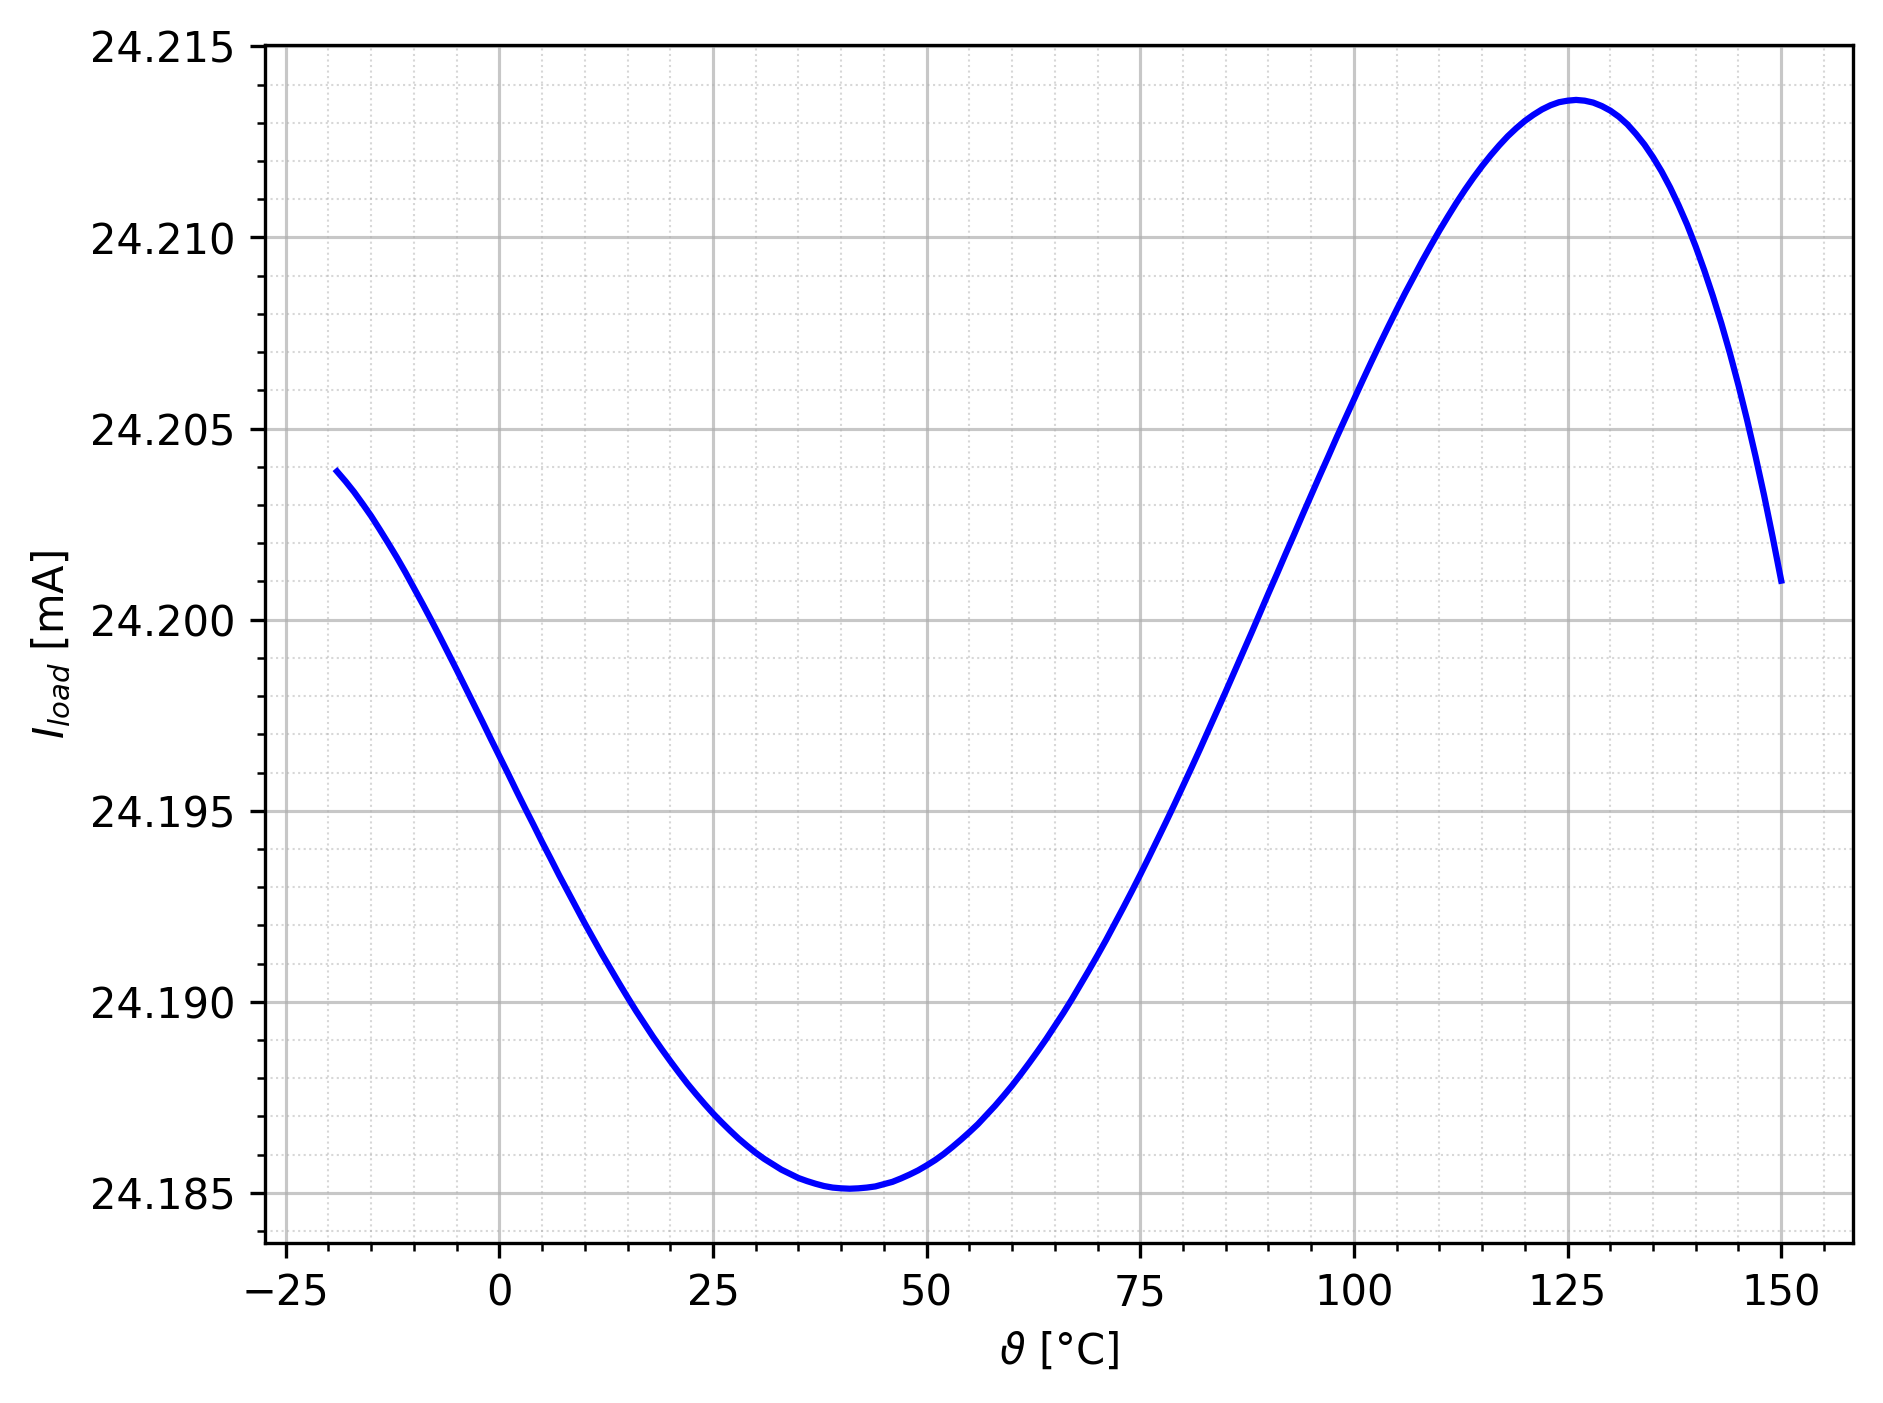
\includegraphics[width=1\linewidth]{Sablona_LaTeX/sim/1a_experiment.png}
            \caption{Teplotní závislost výstupního proudu při~zátěží 100~$\Omega$, při~napájení 5~V a~teplotní závislost napěťové reference LT431 simulována v~programu~LTspice \cite{LTspice}}
            \label{fig:1a_i}
        \end{figure}
        \newpage
        \par
        Kód, pomocí kterého byla tato simulace provedena, je shrnut v~úrývku~\ref{ls:1a}. Pro tuto simulaci byl použit program LTspice \cite{LTspice}.
        \vspace{.5cm}
        \begin{lstlisting}[label=ls:1a,caption=Příkazy využity v~experimentu~1a]
*** PRIKAZY ***
.step temp -20 150 1  ;krokovani parametru globalni teploty
.op                   ;vypocet pracovniho bodu (I(Rload))
        \end{lstlisting}

        \par
        Pro stanovení koeficientu $\theta_{Iout}$ byla provedena numerická derivace knihovnou Numpy pro~jazyk Python \cite{python312,numpy224,pandas223}. Jednoduchý program, který byl pro~tyto účely použit je obsahem úryvku~\ref{ls:num_der}.
        
        \begin{figure}[]
            \centering
            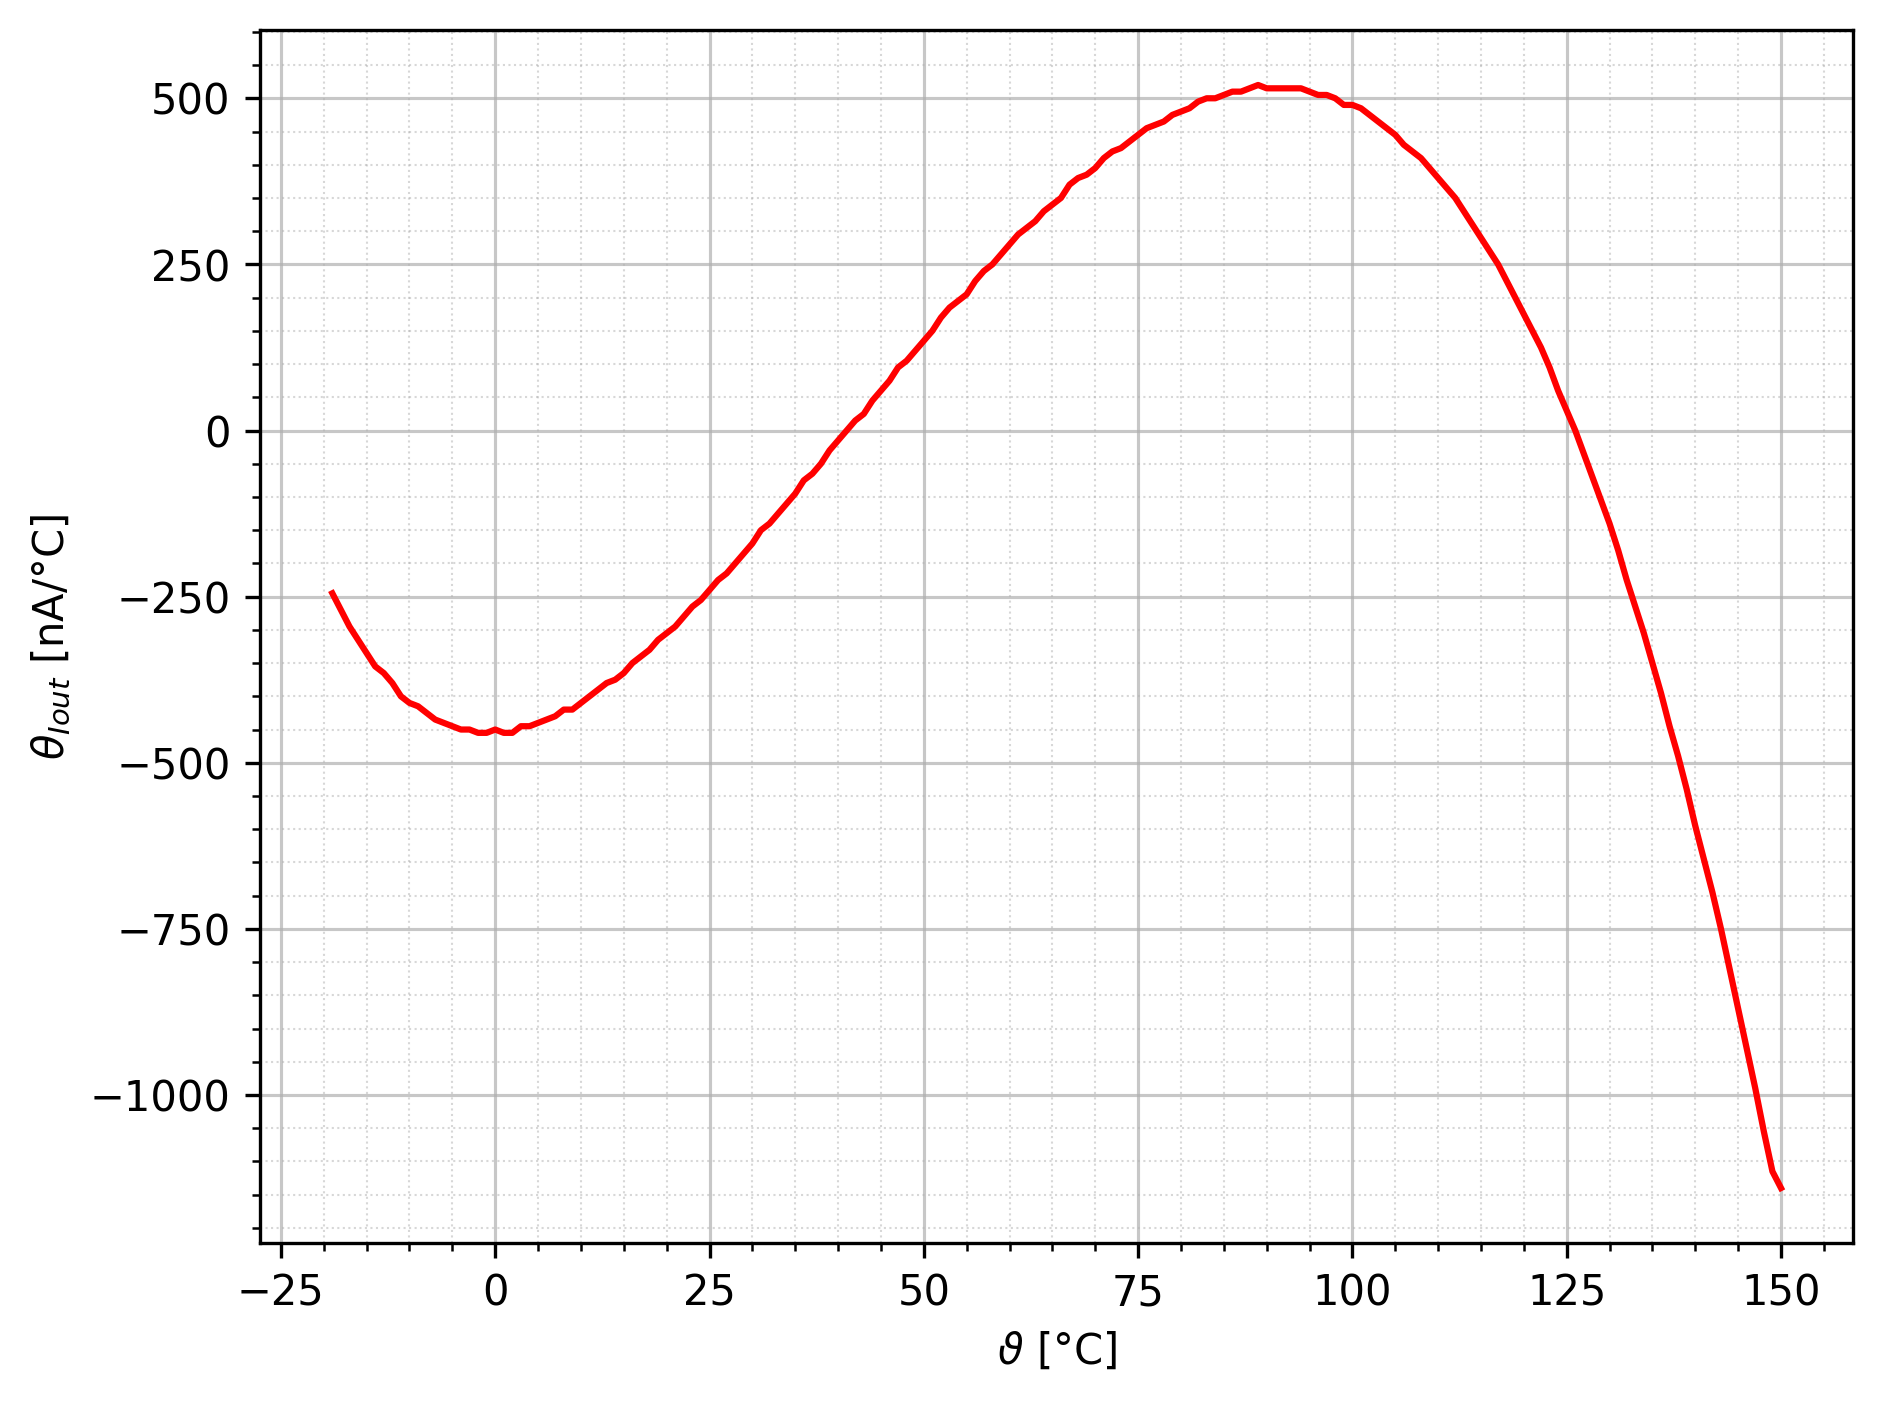
\includegraphics[width=1\linewidth]{Sablona_LaTeX/sim/1a_experiment_theta.png}
            \caption{Derivace závislosti~\ref{fig:1a_i} popisující teplotní závislost teplotního~koeficientu $\theta_{Iout}$}
            \label{fig:1a_theta}
        \end{figure}
        \vspace{.5cm}
        \par
        Z~obrázku je patrné, že nejvyšší hodnoty dosahuje $\theta_{Iout}$ kolem 90~$^\circ$C (přibližně 500~nA/$^\circ$C). Odtud je možno pro odpovídající hodnotu proudu spočíst poměrný teplotní koeficient:
        
        \begin{equation}
            \frac{500\cdot 10^{-9}}{24,2\cdot 10^{-3}}\approx20,661 \text{ ppm/}^\circ\text{C}
        \end{equation}

        \par
        Výrobce přitom uvádí vztah~\ref{eq:TI_alpha} pro teplotní koeficient napěťové reference, který je přímo úměrný výše vyjádřenému koeficientu $\theta_{Iout}$ \cite{TI_TL431_datasheet}. V~tomto vztahu odpovídá veličině $\Delta T_A$ teplotní rozsah aplikace a~$V_{I(dev)}$ rozdíl mezi maximální a~minimální úrovní napětí na~rozsahu teplot $\Delta T_A$.

        \begin{equation}\label{eq:TI_alpha}
            \alpha_{Vref}=\frac{\frac{V_{I(dev)}}{V{ref}\text{ při~25}^\circ\text{C}}\cdot10^6}{\Delta T_A}\text{ [ppm/}^\circ\text{C]}
        \end{equation}

        \par
        Po dosazení získáváme hodnotu:
        \begin{equation}
            \alpha_{Vref} = \frac{\frac{2,4934589-2.4599218}{2.495}\cdot10^6}{170}=79,069\text{ ppm/}^\circ\text{C}
        \end{equation}

        \par
        Výsledek simulace ($\approx$20,5~ppm/$^\circ$C) je tedy v~toleranci stanovené výrobcem \cite{TI_TL431_datasheet}.
        
    \newpage        
    \subsection{Experiment 1b: Maximální hodnota zátěže}\label{subsec:1b}
        Předmětem této části experimentu bylo vyjádřit závislost výstupního proudu na velikosti zátěže a~zároveň zjistit vztah pro maximální hodnotu této zátěže, při níž bude ještě probíhat regulace.
        \par
        Nastavením simulačního programu LTspice byla stanovena velikost odporu $R_S$ na~100~$\Omega$ (pro nastavení výstupního proudu na~hodnotu 25~mA) a~napětí napájecího zdroje na~hodnoty 5~V, 15~V a~36~V (viz~tab.~\ref{tab:max_ratings}), nakonec byla měněna velikost odporu $R_{load}$, a~to mezi hodnotami 5~$\Omega$ až~10~k$\Omega$ (viz~úryvek~\ref{ls:1b}) \cite{LTspice}. Výsledek této simulace je obsahem obrázku~\ref{fig:1b}

        \begin{lstlisting}[label=ls:1b,caption=Příkazy využity v~experimentu~1b]
*** PRIKAZY ***
.op  ;vypocet pracovniho bodu
.step param valrload 5 10k 100  ;krokovani velikosti zateze
.step param vccval list 5 15 36 ;krokovani hodnoty napajeni
        \end{lstlisting}
        
        \begin{figure}[h]
            \centering
            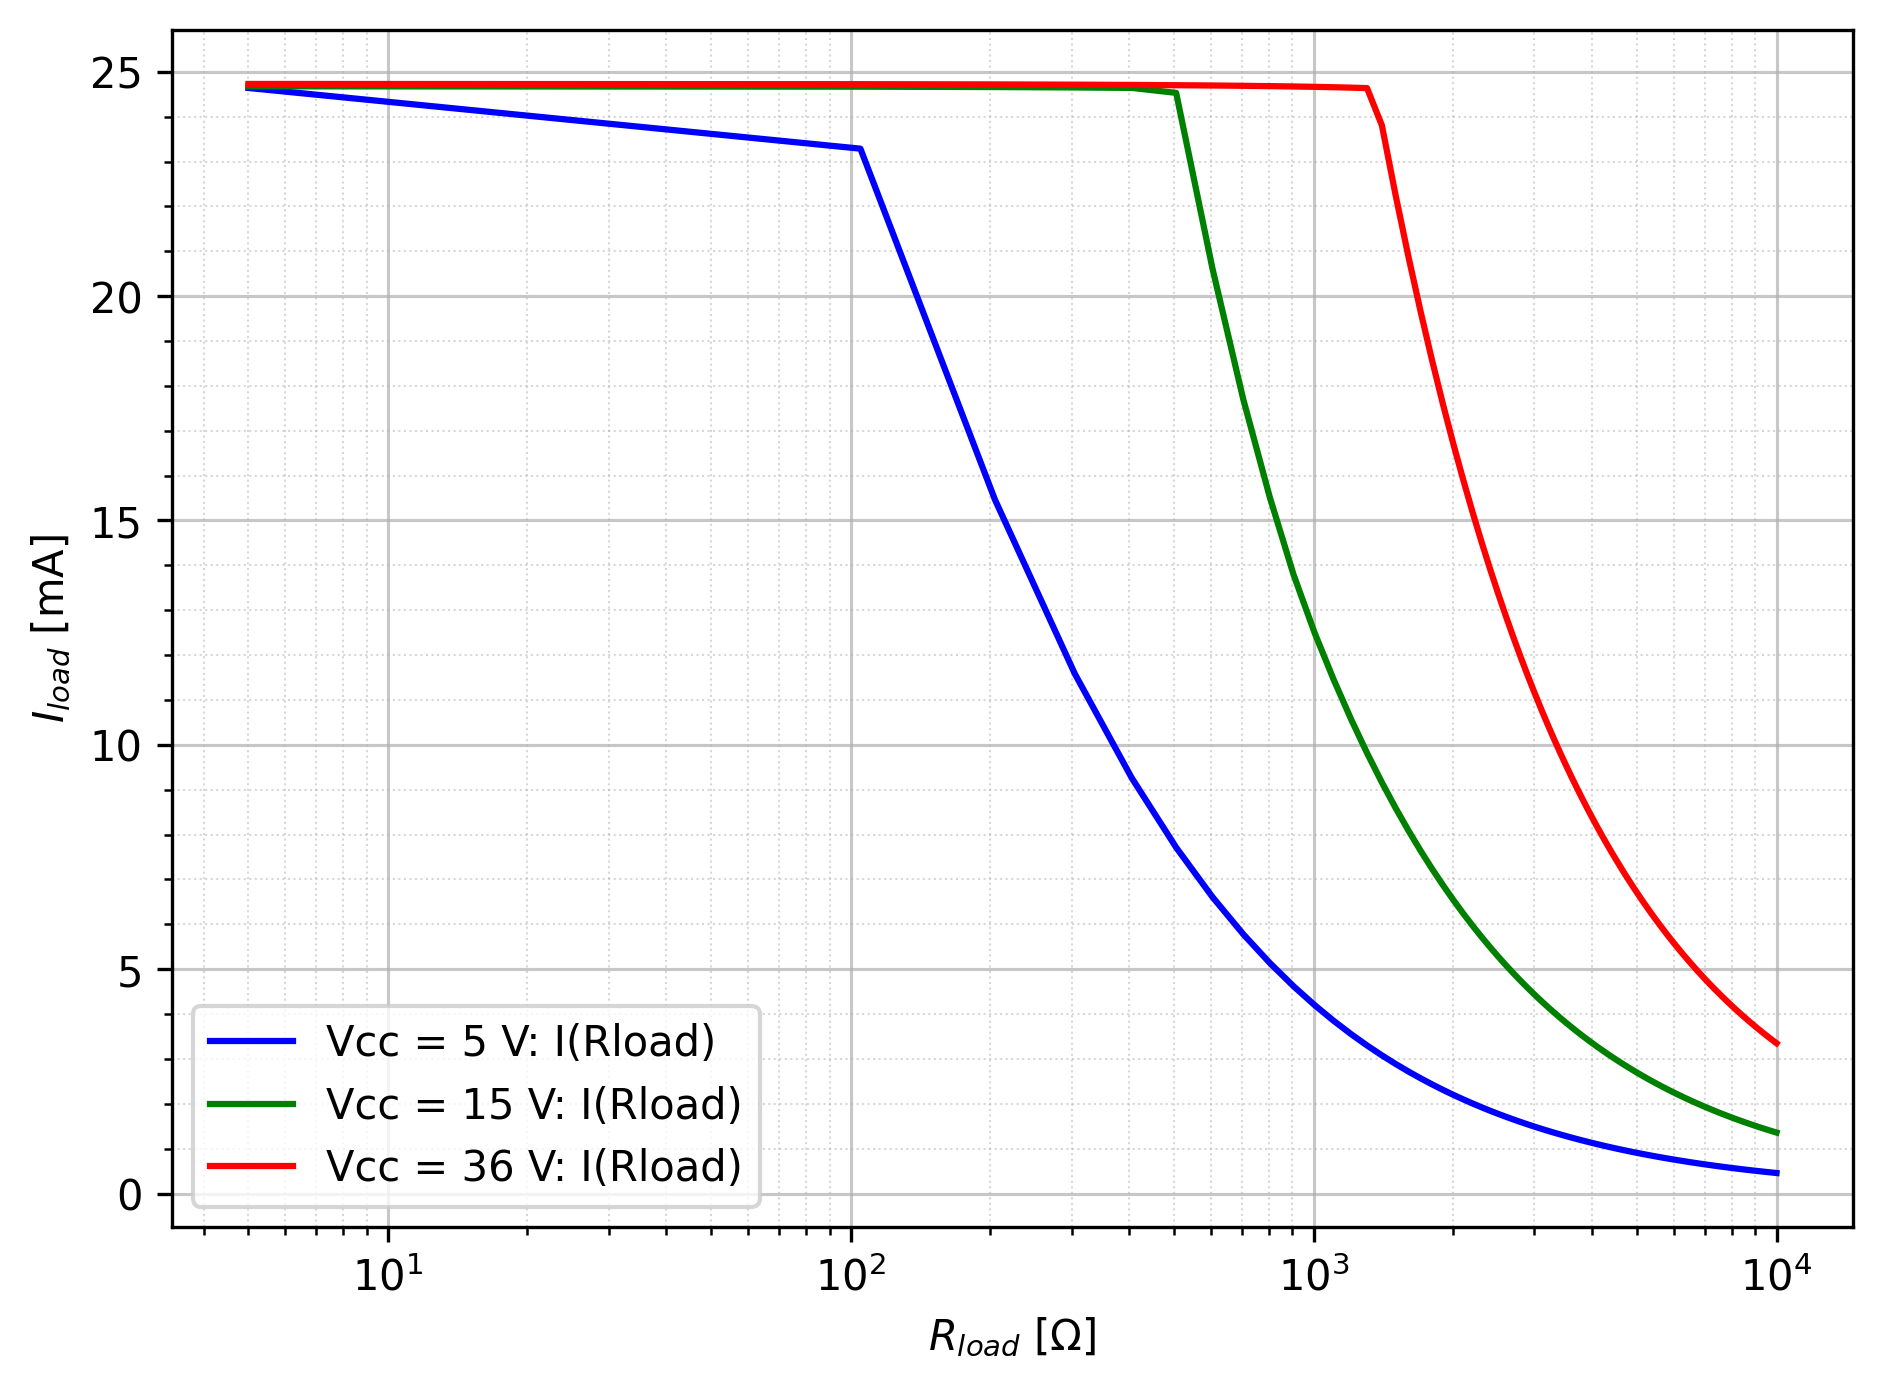
\includegraphics[width=1\linewidth]{Sablona_LaTeX/sim/1b_experiment.png}
            \caption{Závislost proudu zátěží na~velikosti zátěže a~napájecím napětí simulována v~prostředí LTspice \cite{LTspice}}
            \label{fig:1b}
        \end{figure}
    
        \par
        U~výrazných poklesů na~obrázku je patrný lineární trend hodnoty $R_{load}$, při~níž~tento zlom nastává, v~závislosti na~napětí Vcc. Z~analýzy simulovaného obvodu vyplývá vztah:
        \begin{equation}\label{eq:Rmax}
            V_{ka}=V_{CC}-R_{load}I_{out},
        \end{equation}
        kde $V_{ka}$ je katodové napětí \cite{Svoboda2014}. Po dosazení získáváme pro napájecí napětí 5~V a~katodové napětí 2,495~V hodnotu $R_{load}^{max}$:
        \begin{equation}
            R_{load}^{max} = \frac{15-2,495}{25\cdot 10^{-3}} = 500,2\text{~}\Omega.
        \end{equation}

        \par
        Po dosazení pro napájecí napětí, jež byla použita při krokování v~simulaci, získáváme hodnoty $R_{load}^{max}$ odpovídající těm z~grafické závislosti (tab.~\ref{tab:1b}). Jelikož jsou tyto hodnoty charakteristické pro~simulované zapojení, nelze je srovnávat s~technickým listem.

        \begin{table}[]
        \centering
        \caption{Maximální hodnoty zátěže pro vybrané napájecí napětí při regulaci $I_{out}$ na~25~mA}
        \label{tab:1b}
        \begin{tabular}{cc}
        \textbf{Vcc {[}V{]}} & \textbf{$\mathbf{R_{load}^{max}} \textbf{~[}\Omega\textbf{]}$} \\ \hline
        5                    & 100,2                     \\
        15                   & 500,2                     \\
        36                   & 1340,2                   
        \end{tabular}
        \end{table}
    
    \newpage    
    \subsection{Experiment 2: Šumová analýza}\label{subsec:2}
        Pro provedení šumové analýzy byl obvod popsán v~programu PSpice, jelikož oproti LTspice disponuje lepšími nástroji pro tuto analýzu \cite{pspice}. Pracovní bod byl nastaven tak, aby při linearizaci obvodu v~rámci AC analýzy, potřebné pro šumovou, byl tento proces proveden v~oblasti regulace. Hodnota $R_S$ byla zvolena jako 250~$\Omega$ pro výstupní proud 10~mA a~napájecí napětí bylo nastaveno na~19,1~V. Celý soubor popisující obvod je shrnut v~kódu~\ref{ls:2}.

        \hspace{2cm}

        \begin{lstlisting}[label=ls:2,caption=Obsah souboru .cir pro experiment 2]
* uzel 'in' byl prejmenovan na '3' z duvodu chyby .noise

*** NETLIST ***
Vcc 	3    {VCC}     AC {VCC}
Rb      3    kat       1k
Rload   aux3 col       100
Rs      ref  0 	       250
Xref 	ref  0    kat  TL431
Q1      col  kat  ref  Q2N2222

Vload 3 aux3 0

*** PRIKAZY ***	
.lib tl431.mod
.lib MPS.lib
.param VCC = 19.1
.op
.ac dec 1000 1 150k  ;ac analyza pro tisic bodu
.noise V(3,col) Vin
.probe
.end
        \end{lstlisting}
        \hspace{.5cm}

        Pomocí postprocesoru .probe byly vykresleny frekvenční závislosti hustoty šumového výkonu a~napětí (obr.~\ref{fig:2_a}) a~také efektivní hodnota šumového proudu (obr.~\ref{fig:2_b}).
        \par
        Ačkoliv je vztah mezi spektrální hustotou šumového výkonu a~proudu charakterizován mocninou dvěma \cite{prednasky}, není patrná jakákoliv transformace průběhů závislostí z~obrázku~\ref{fig:2_a}. Je to z~důvodu, že hodnoty obou výstupních parametrů jsou na~kmitočtu v~simulované oblasti téměř nezávislé, a~tak se odmocnění téměř neprojeví na~průběhu.
        \par
        Takto konstantní průběh je překvapivý, a~to především ve~srovnání s~průběhem, jenž popisuje výrobce (obr.~\ref{fig:TL431_noise}). Ačkoliv se jedná o~spektrální hustoty šumového napětí, měl by být průběh vycházející ze~simulace totožný (je totiž normalizován na~odpor 1~$\Omega$)~---~přitom byly parametry pro toto měření nastaveny shodně s~těmi, jež poskytl výrobce \cite{TI_TL431_datasheet}.

        \begin{figure}[h]
            \centering
            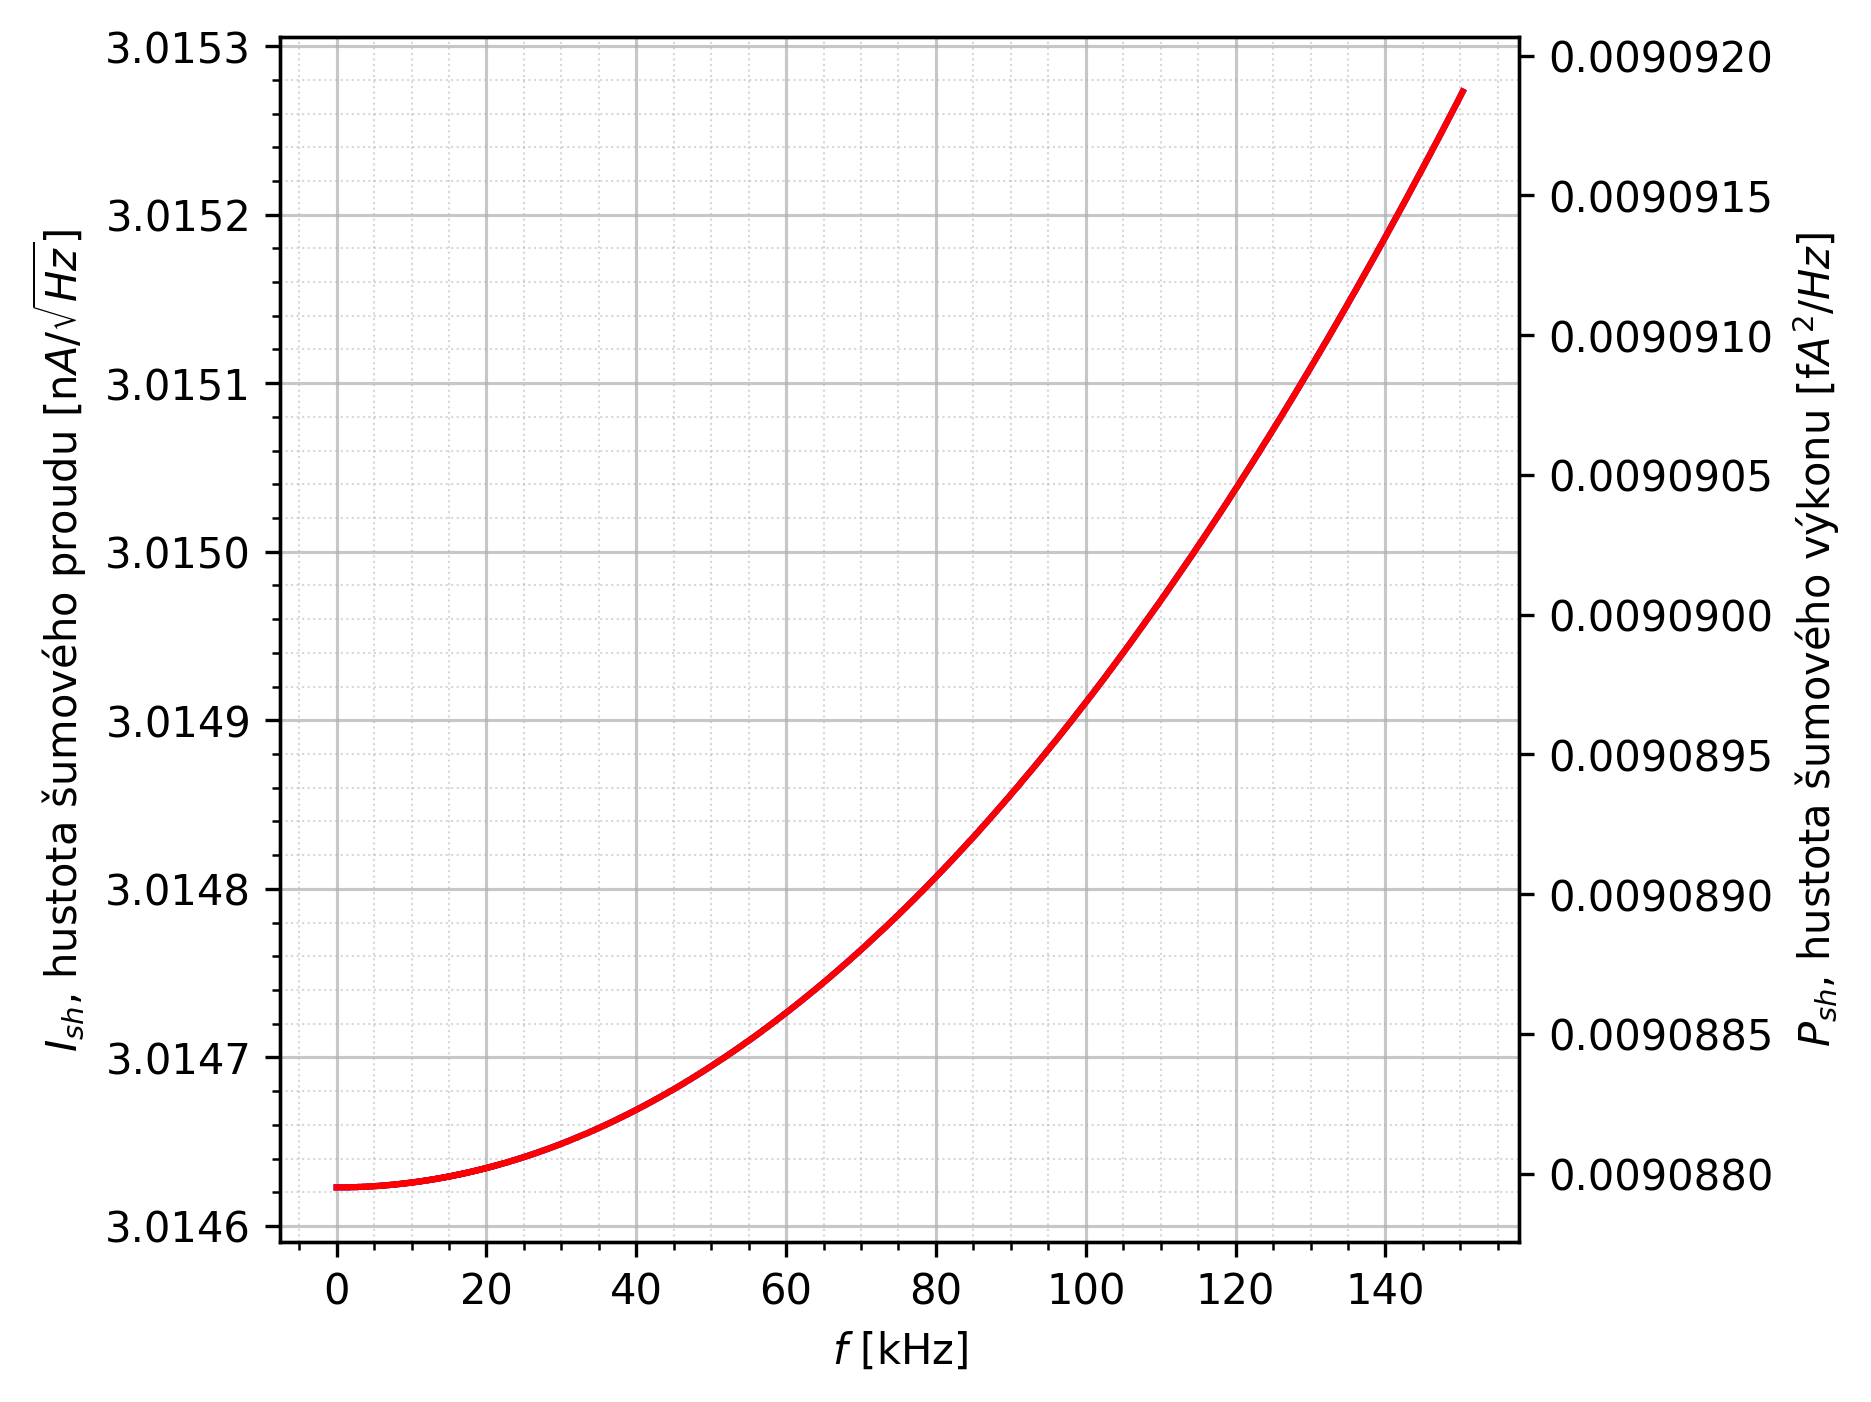
\includegraphics[width=1\linewidth]{Sablona_LaTeX/sim/2_experiment_Ish_Psh.png}
            \caption{Kmitočtová charakteristika spektrální hustoty šumového výkonu a~proudu~\cite{pspice}}
            \label{fig:2_a}
        \end{figure}
        
        \begin{figure}[h]
            \centering
            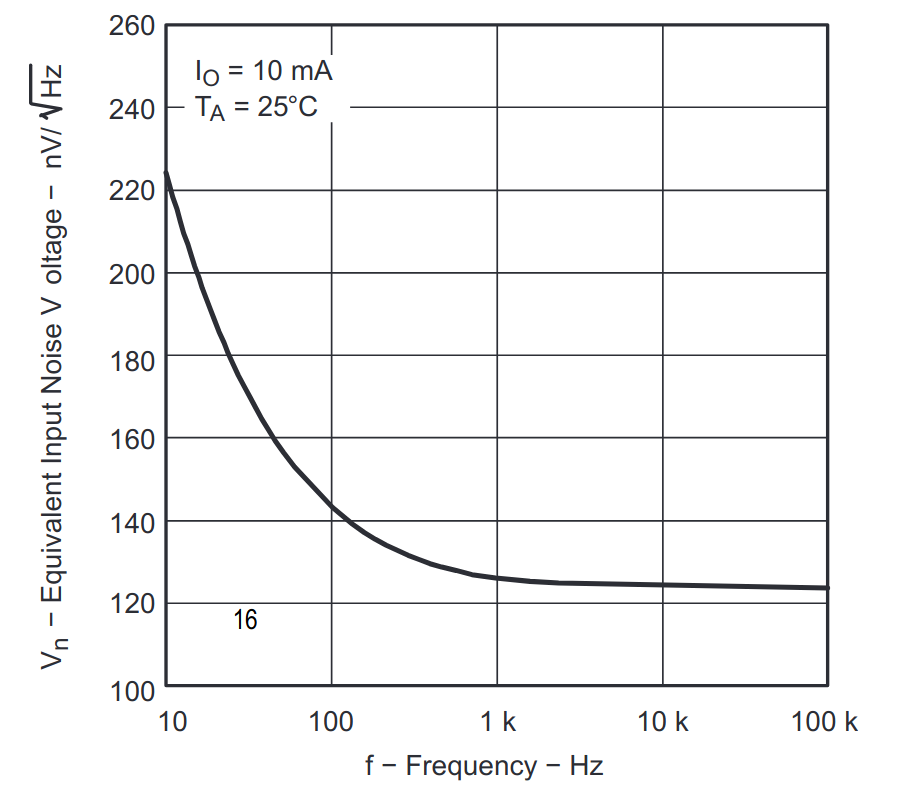
\includegraphics[width=0.65\linewidth]{Sablona_LaTeX/obrazky/TL431_noise.png}
            \caption{Kmitočtová charakteristika spektrální hustoty šumového napětí TL431 poskytnuta výrobcem \cite{TI_TL431_datasheet}}
            \label{fig:TL431_noise}
        \end{figure}
        \clearpage
        \newpage
        \par
        Hodnota proudu zátěží se na~nízkých kmitočtech blíží hodnotě 20~$\mu$A, ale již při 90~kHz překračuje hranici 1~\% výstupního proudu (100~$\mu$A) a~při kmitočtu 150~kHz dosahuje téměř 250~$\mu$A (tedy 2,5~\%). Kolem 1~kHz je poměr šumového proudu ku~proudu zátěží (resp. jeho citlivosti na~malý signál) nejhorší (viz~obr.~\ref{fig:pomer}). Přesto však dosahuje pouze 1,2~\%. Srovnání absolutních hodnot efektivního šumového proudu s proudem v~pracovním bodě je tudíž bezpředmětné.

        \vspace{3 cm}
        
        \begin{figure}[h]
            \centering
            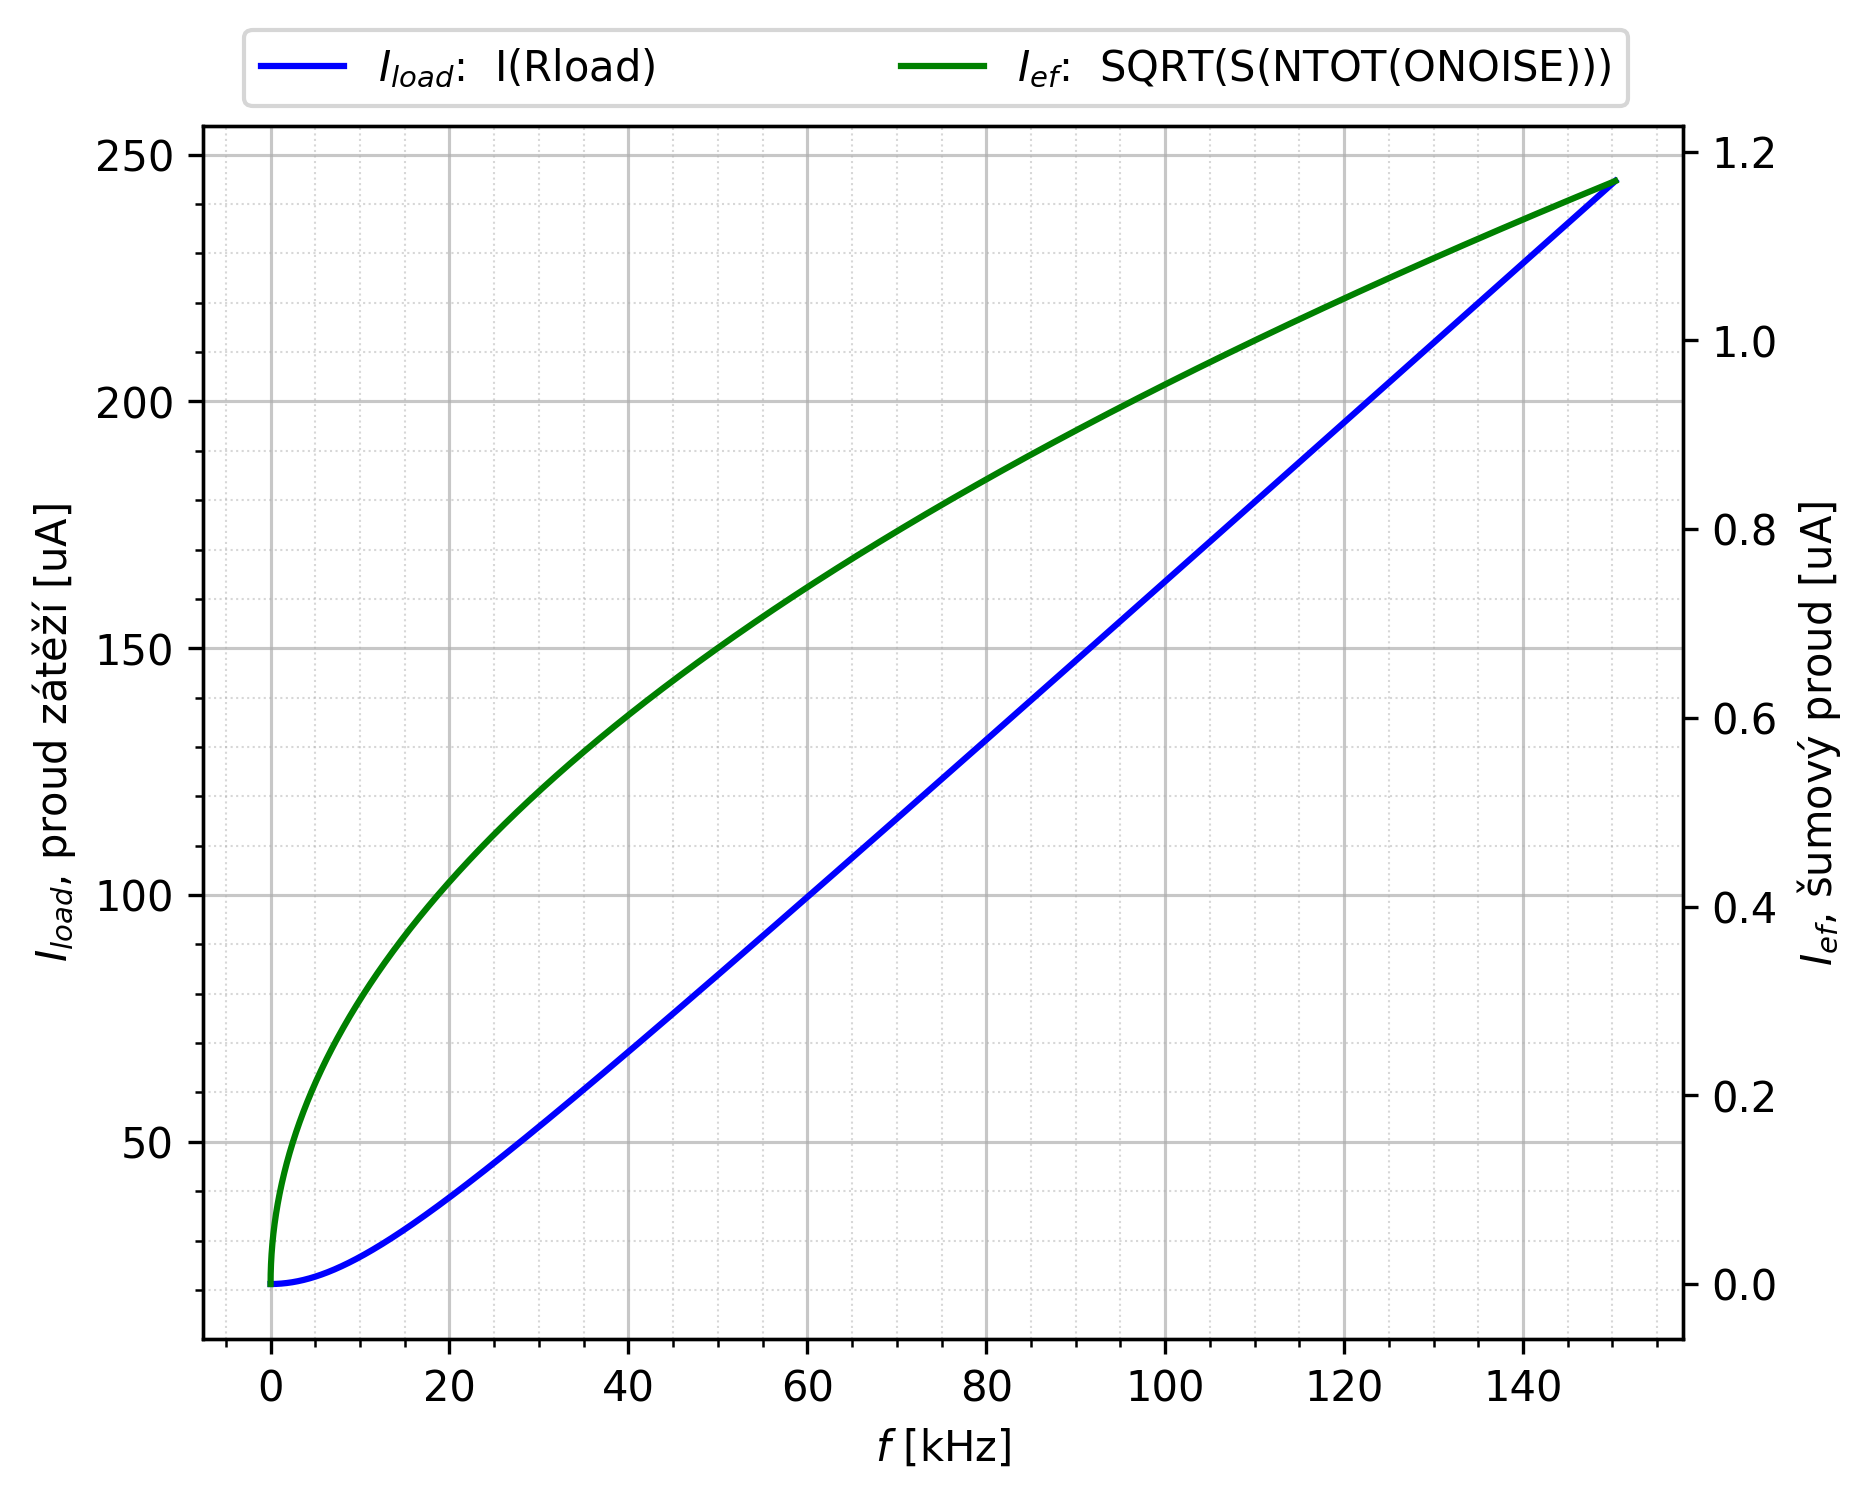
\includegraphics[width=\linewidth]{Sablona_LaTeX/sim/2_experiment_irload_ief.png}
            \caption{Kmitočtová charakteristika efektivní hodnoty šumového proudu ve~srovnání s proudem zátěží \cite{pspice}}
            \label{fig:2_b}
        \end{figure}

        \newpage
        \par
        Charakteristika spektrální hustoty šumového napětí, resp. proudu, poskytnuta výrobcem, jeví charakteristický průběh pro polovodičové součástky v~důsledku přítomnosti tzv. 1/F, neboli blikavého, šumu \cite{prednasky}. Protože je tato vlastnost u~simulovaného průběhu nepřítomna, lze~se~domnívat, že se jedná o~nepřesnost modelu, jež je podle rozboru kapitoly~\ref{sec:rozhrani} sestavena za~pomocí řízeného zdroje napětí, a~tak mohou být některé polovodičové vlastnosti této součástky zanedbány.

        \vspace{2 cm}
        
        \begin{figure}[h]
            \centering
            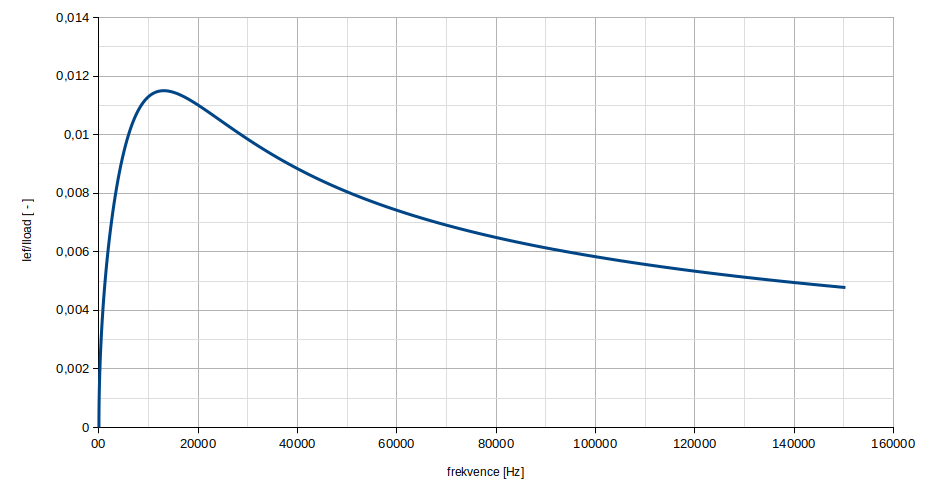
\includegraphics[width=\linewidth]{Sablona_LaTeX/sim/pomer.png}
            \caption{Poměr efektivní hodnoty šumového napětí a~proudu zátěží v~závislosti na~kmitočtu \cite{pspice}}
            \label{fig:pomer}
        \end{figure}
    \clearpage
    \newpage
    \subsection{Experiment 3: Pulzní odezva}\label{subsec:3}
        V~rámci zkoumání pulzní odezvy obvodu (resp. součástky TL431, která je pro tuto funkci klíčová) byla využita transientní (neboli časová) analýza \cite{Krejcirik2001}. Obsah souboru .cir, jež byl pro simulaci použit je předmětem úryvku kódu~\ref{ls:3} (napsán pro simulační prostředí PSpice \cite{pspice}).
        \vspace{.5 cm}
        \begin{lstlisting}[label=ls:3,caption=Obsah souboru .cir pro experiment 3]
*** NETLIST ***
Vin     3    0    5    PULSE 0 5 1u 1f 1f 5u 10u
Rb      3   kat  1k
Rload   3    col  100
Rs      ref  0    100 ;Iout = Vref / Rs -> Rs = 2.5/25m
Xref    ref  0    kat TL431
Q1      col  kat  ref Q2N2222

*** PRIKAZY ***
.tran 8n 8u 0 10u SKIPBP
.lib tl431.mod
.lib MPS.lib
.probe
.op
.end
        \end{lstlisting}

        \par
        Výrobce napěťové reference sám poskytuje charakteristiku pulzní odezvy, kdy je vstupním signálem obdélníkový impuls 5~V o~šířce 5~$\mu$s (viz~obr.~\ref{fig:TL431_pulse}). Simulace byla těmto podmínkám nastavena co~nejblíže. Jejím výstupem je potom průběh na~obr.~\ref{fig:pulse_sim}, jehož detail je na~obr.~\ref{fig:pulse_min_detail}.
        \begin{figure}[h!]
            \centering
            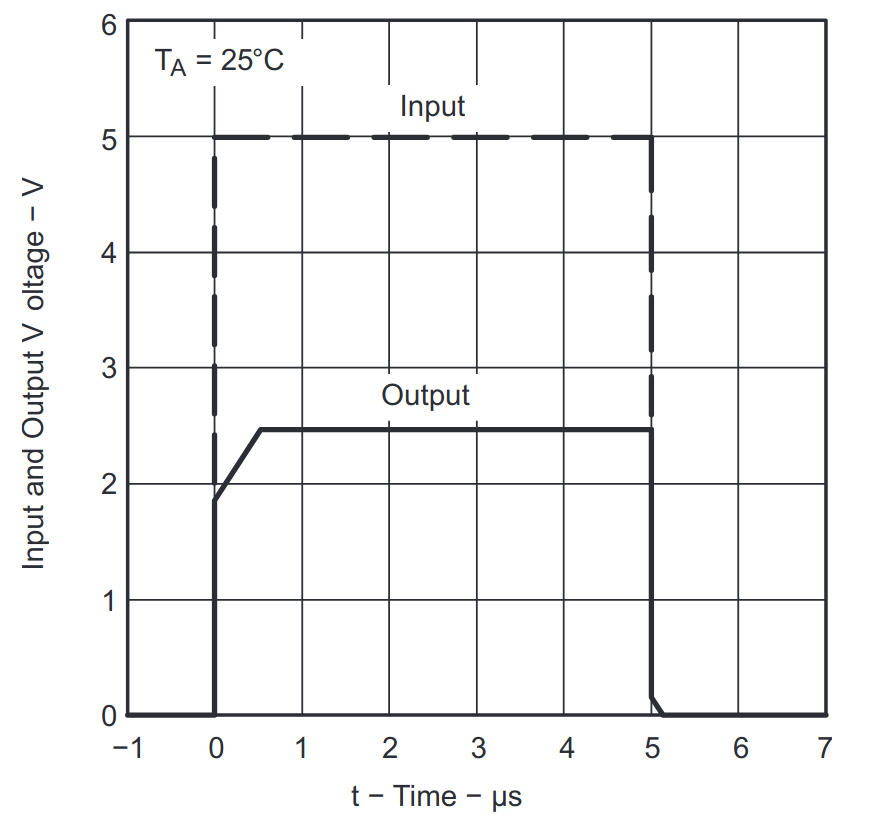
\includegraphics[width=0.5\linewidth]{Sablona_LaTeX/obrazky/TL431_pulse-response.png}
            \caption{Pulzní odezva součástky (referenčního napětí) TL431~poskytnuta~výrobcem \cite{TI_TL431_datasheet}}
            \label{fig:TL431_pulse}
        \end{figure}
        
        \newpage

        \begin{figure}[h]
            \centering
            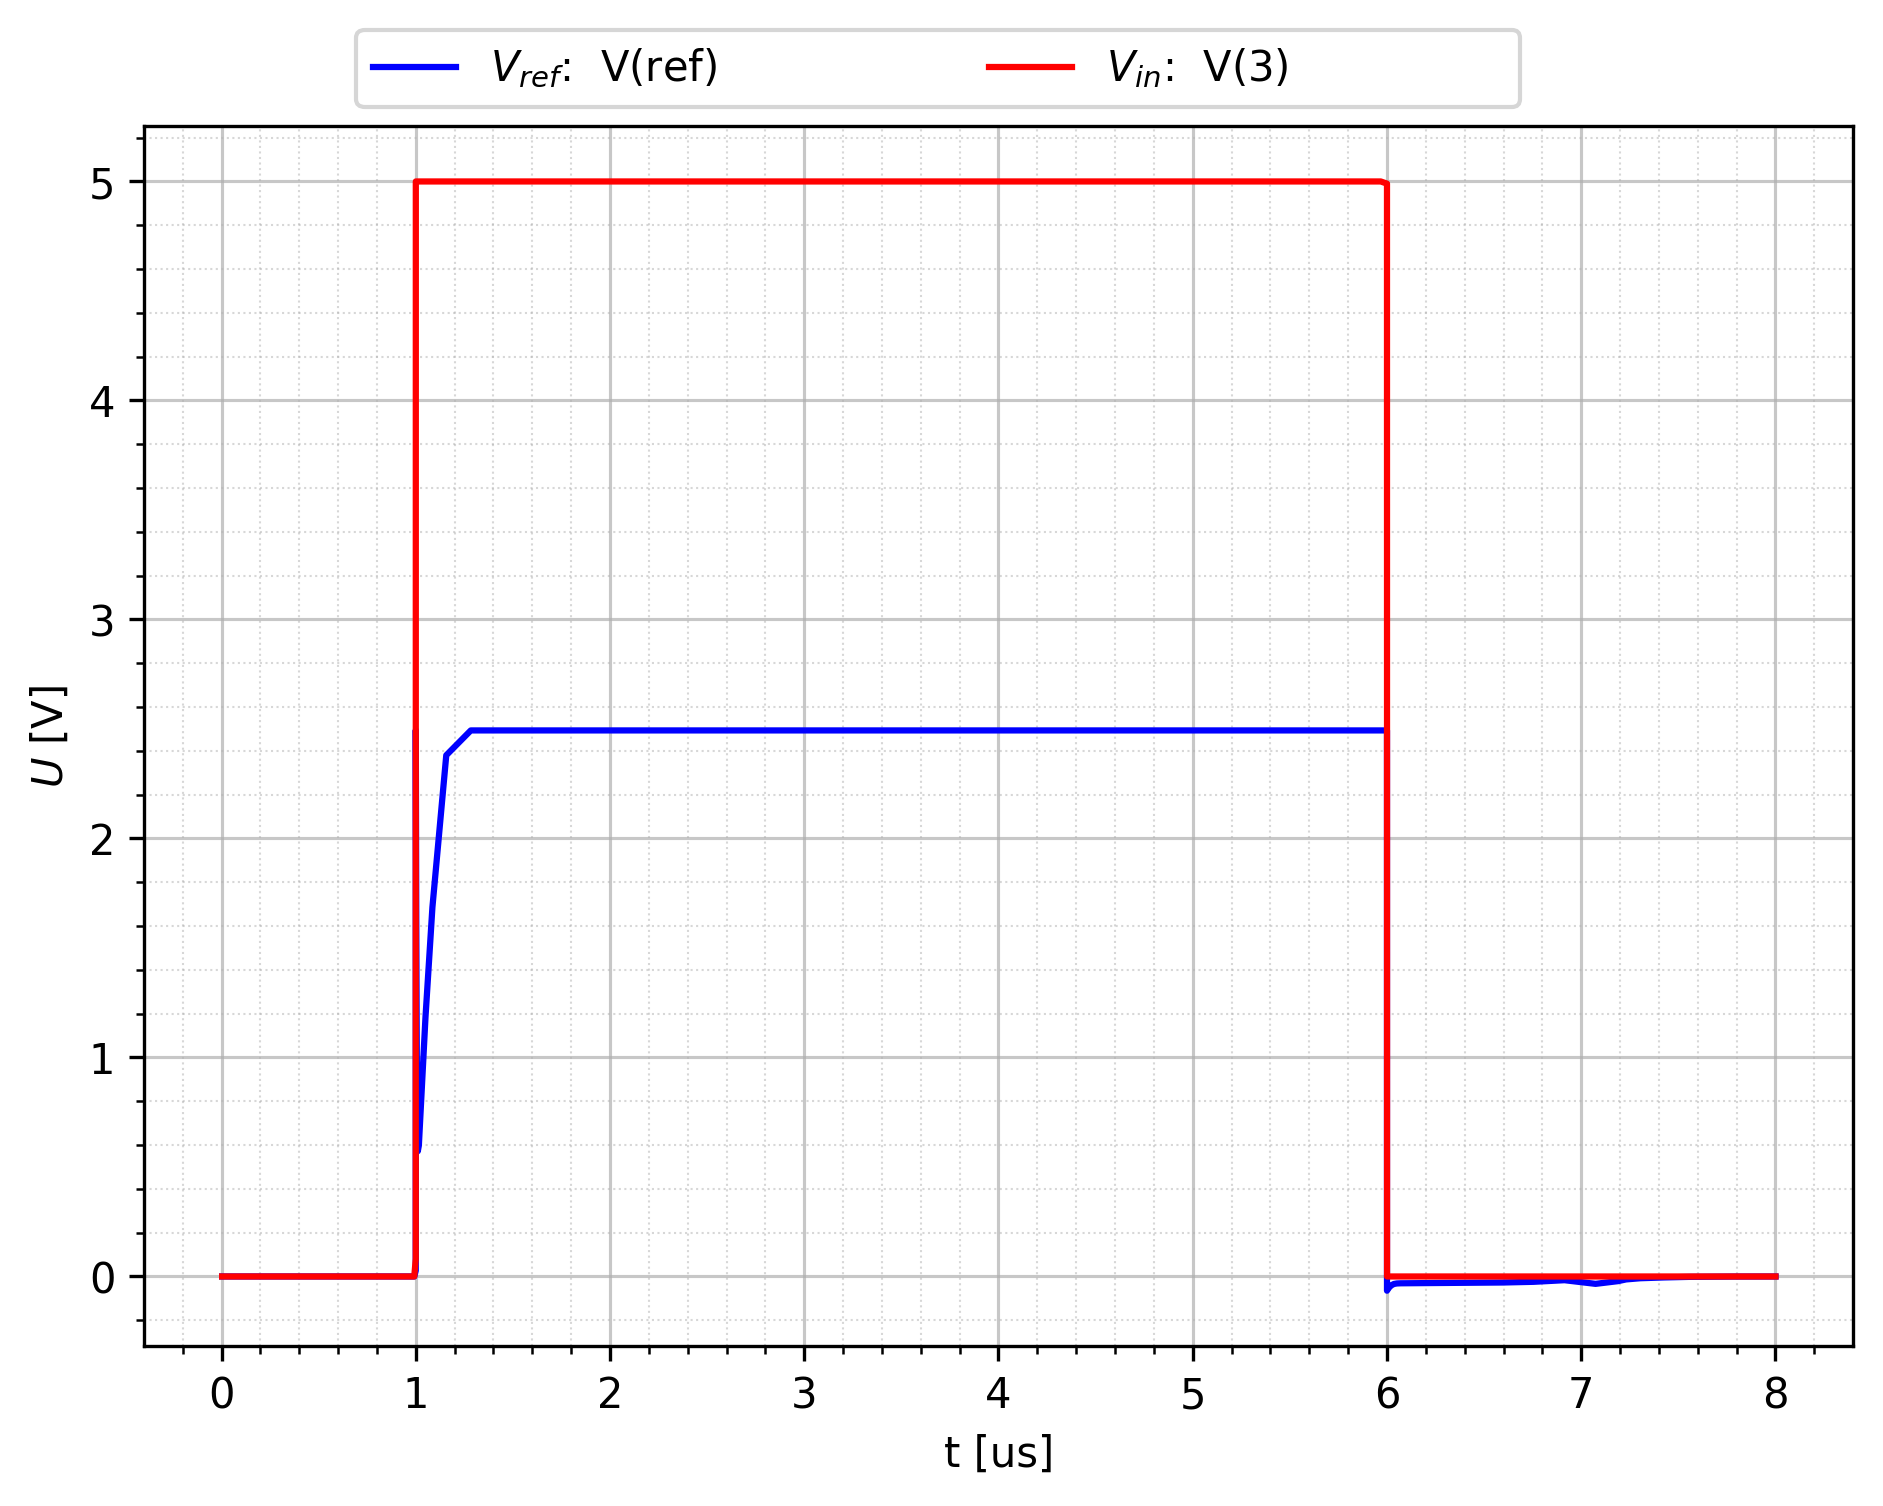
\includegraphics[width=1\linewidth]{Sablona_LaTeX/sim/3_experiment.png}
            \caption{Pulzní odezva součástky (referenčního napětí) TL431 v~simulovaném~obvodu \cite{pspice}}
            \label{fig:pulse_sim}
        \end{figure}

        \begin{figure}[hb!]
            \centering
            \begin{subfigure}[b]{0.45\textwidth}
                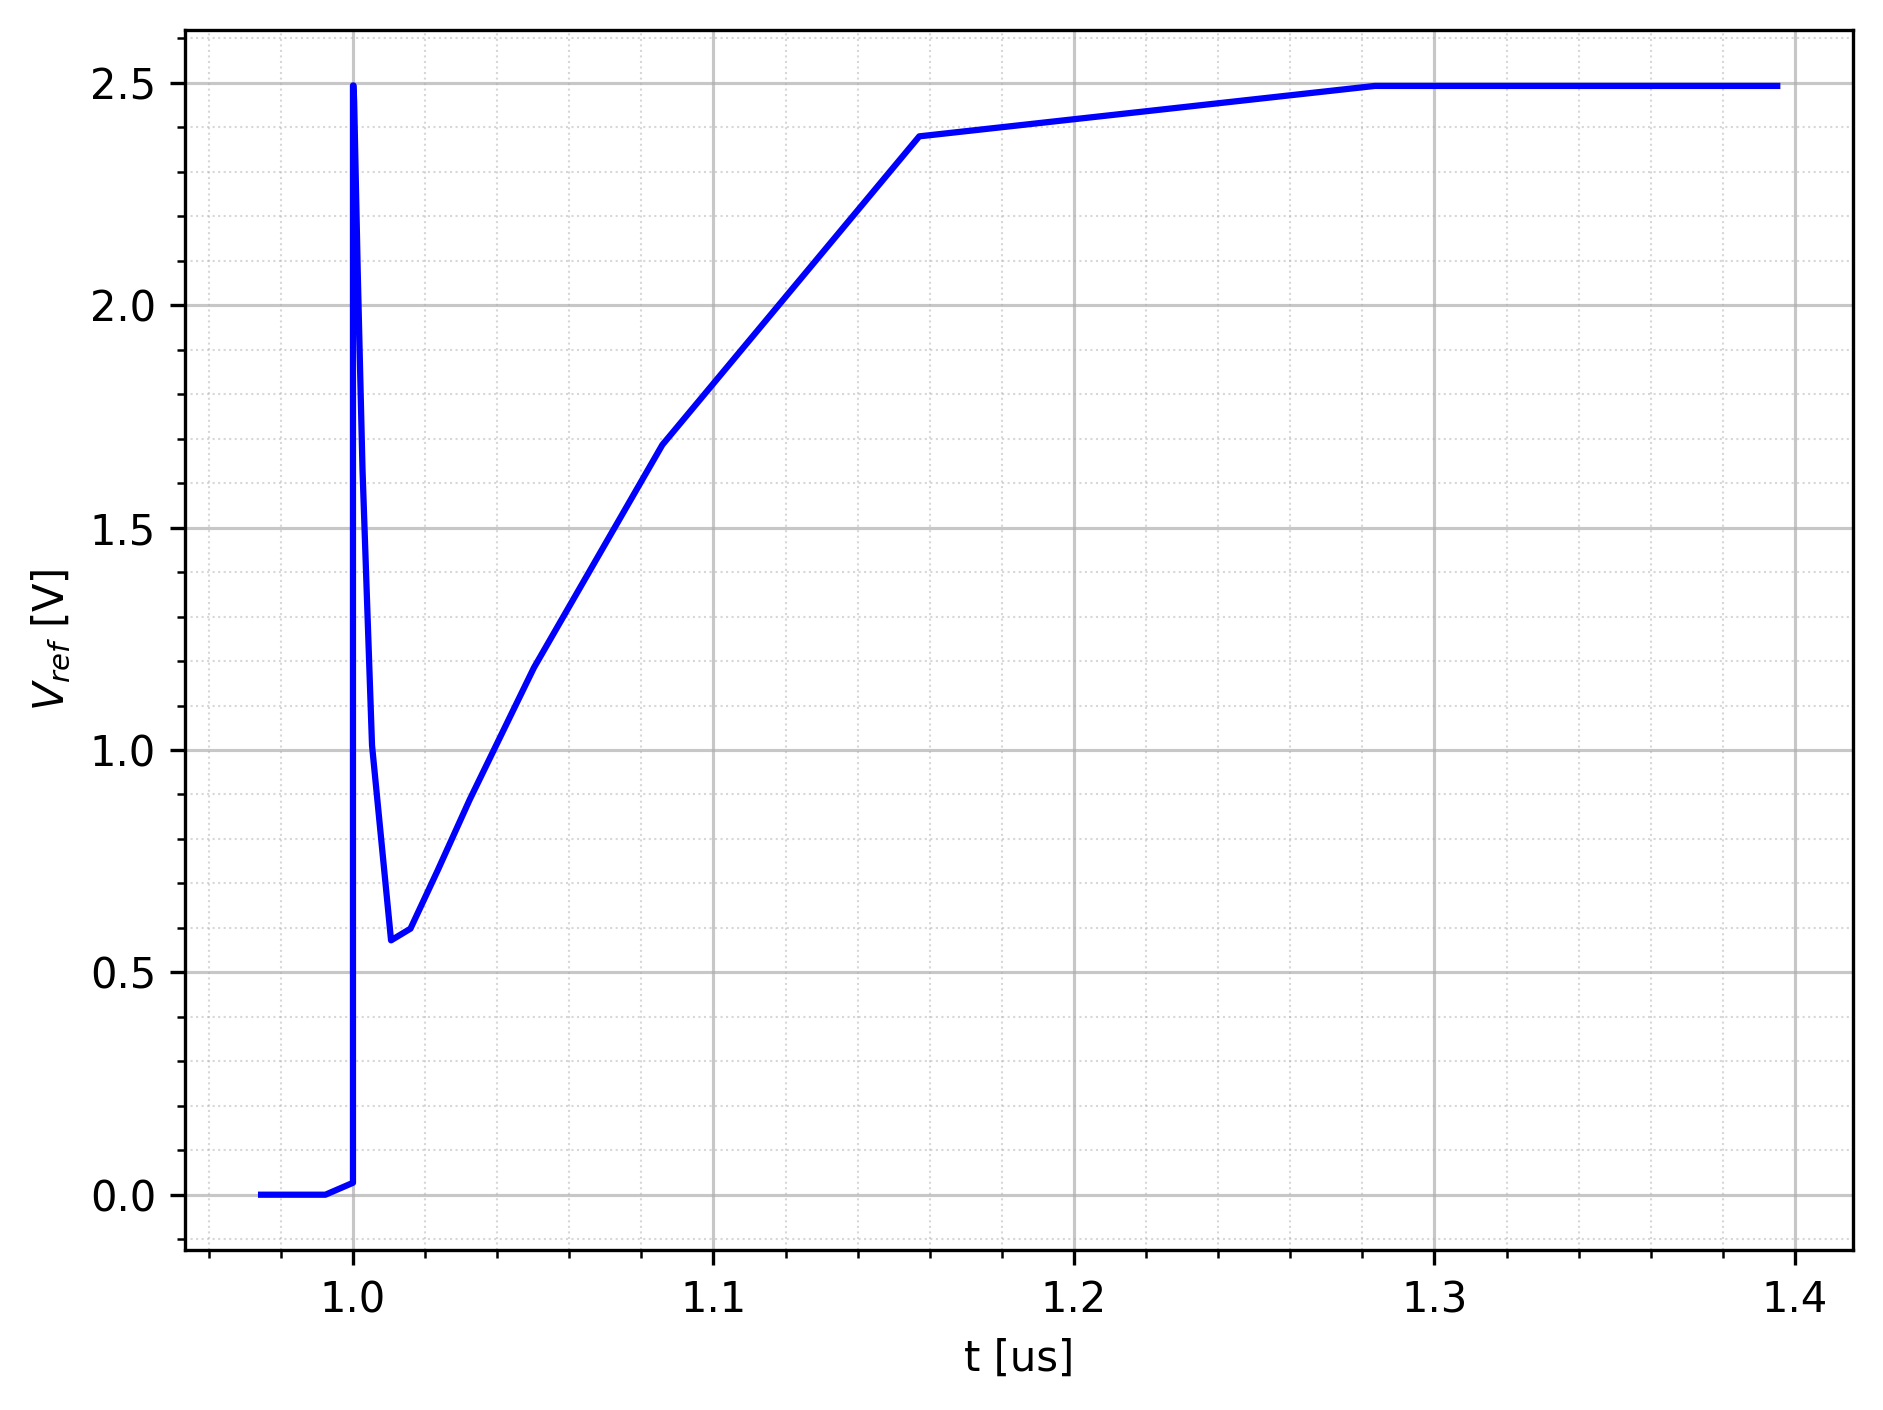
\includegraphics[width=\linewidth]{Sablona_LaTeX/sim/3_experiment_rise.png}
                \caption{Odezva na~náběžnou hranu}
            \end{subfigure}
            \begin{subfigure}[b]{0.45\textwidth}
                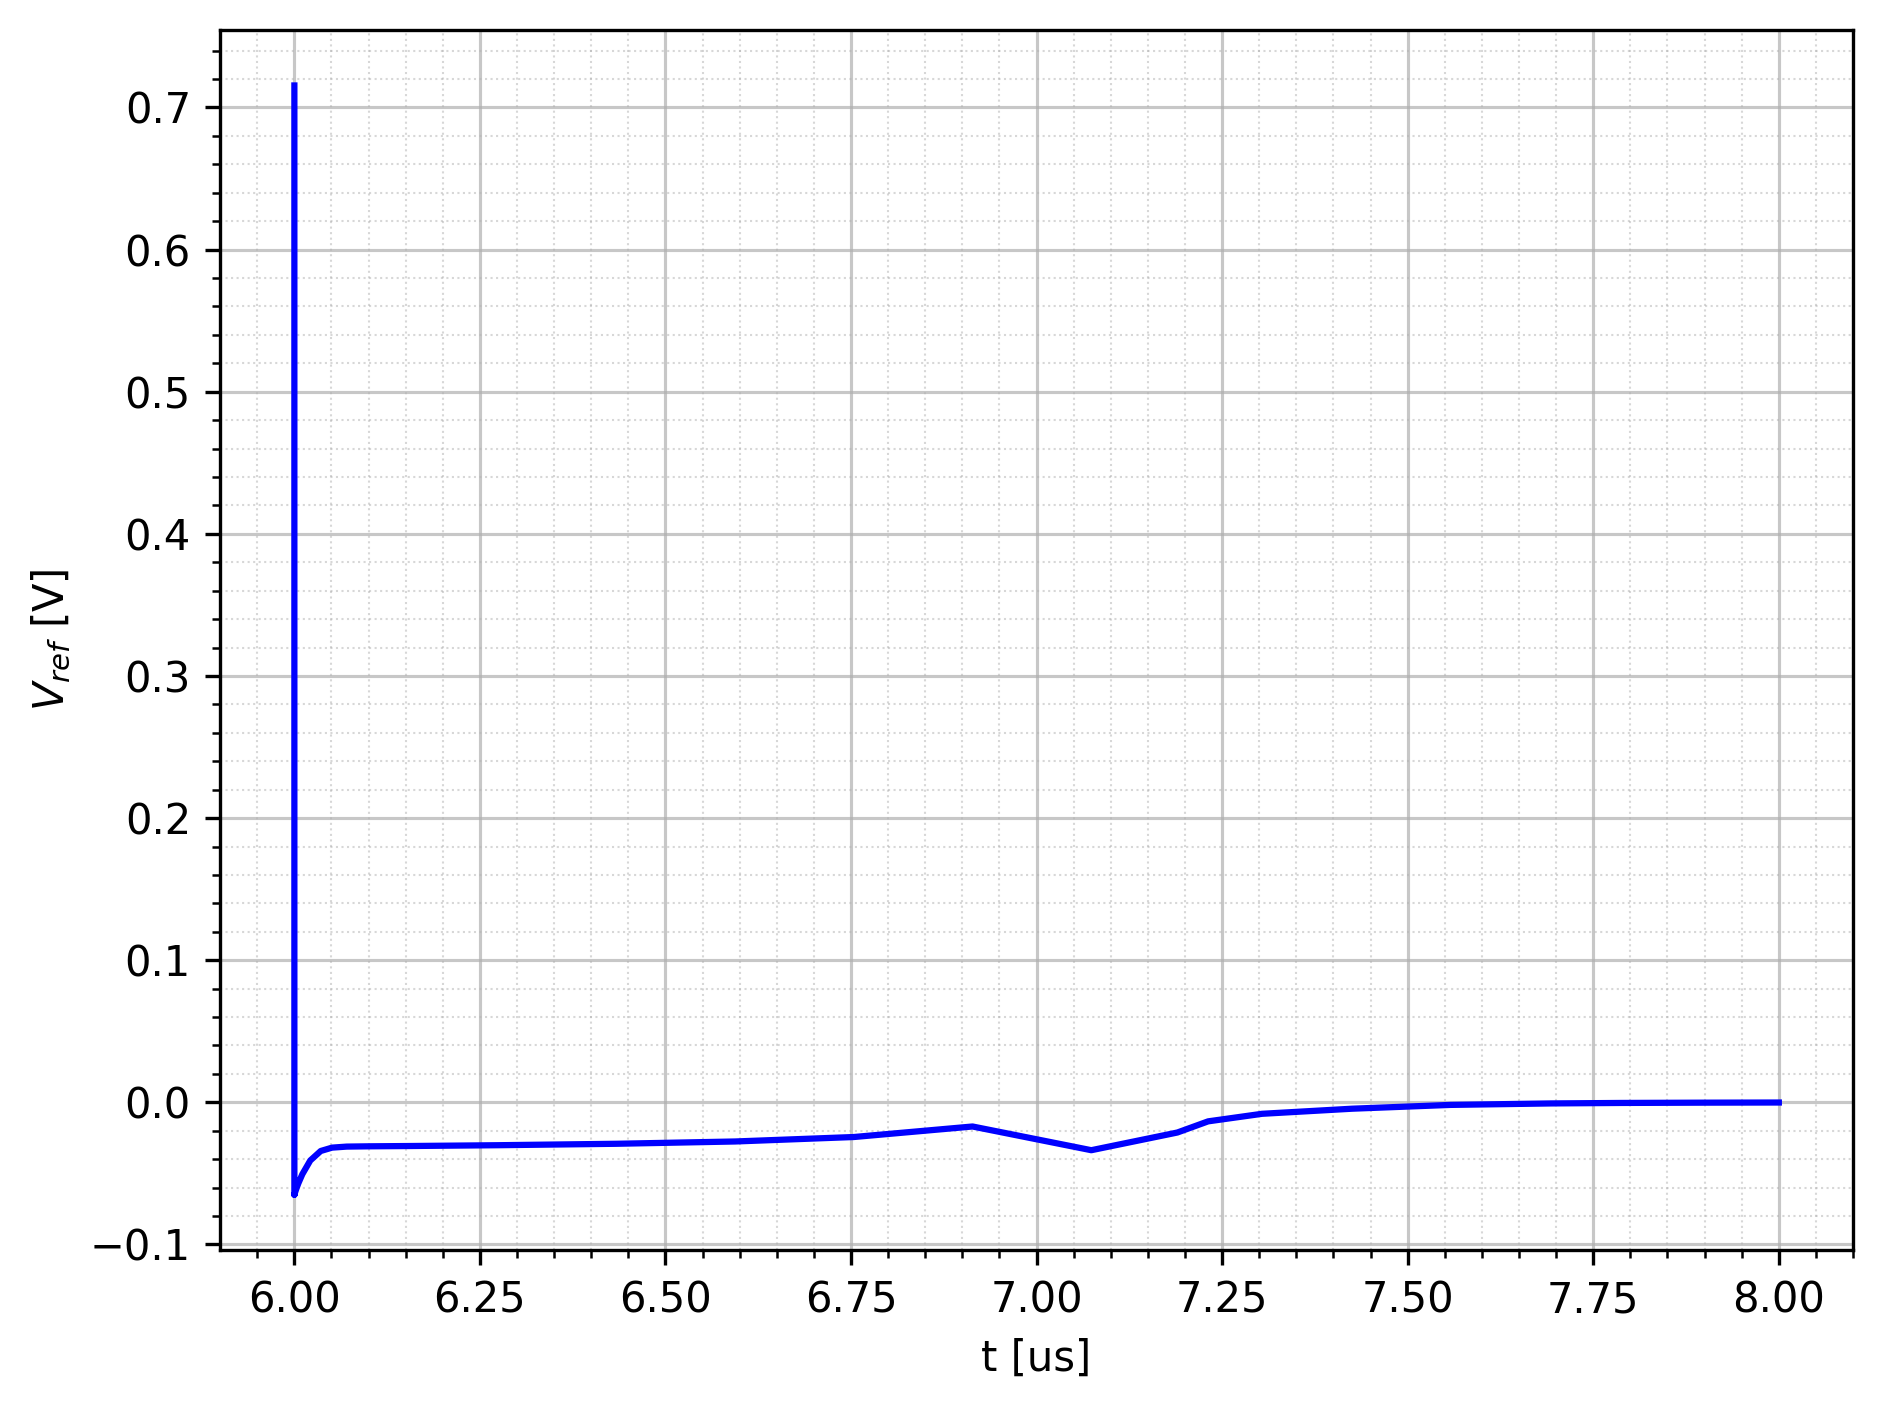
\includegraphics[width=\linewidth]{Sablona_LaTeX/sim/3_experiment_fall.png}
                \caption{Odezva na~sestupnou hranu}
            \end{subfigure}
            \caption{Detail průběhu pulzní odezvy součástky (referenčního napětí) TL431 v~simulovaném~obvodu \cite{pspice}}
            \label{fig:pulse_min_detail}
        \end{figure}
        
        \newpage
        
        \par
        Z~tohoto detailu je patrné, že se výstupní signál v~reakci na náběžnou hranu ustálí již v~čase $\sim$350~ns, přičemž výrobce tuto hodnotu stanovuje na~$\sim$500~ns. Iniciální vrchol průběhu $V_{ref}$ však výrobce neuvádí. Stejně tak není v~technickém listu znázorněna ustalovací doba v~reakci na sestupnou hranu, zatímco z~výstupu simulace jsou patrny fluktuace ve~výstupním napětí ještě celou $\mu$s po pádu vstupní sestupné hrany \cite{TI_TL431_datasheet}.
        \par
        Důvodem těchto jevů může být zapojení, v~němž byla součástka TL431 simulována, jelikož se liší od~zapojení, jež pro tento experiment uvedl výrobce (obr.~\ref{fig:TL431_pulse_cir}). Možnou příčinou prvotního vrcholu může být příliš rychlé \uv{otevření} tranzistoru Q1 (v~technickém listu je jeho časová prodleva uvedena v~řádu desítek~ns, což by tomuto vrcholu odpovídalo). Dlouhá doba ustalování po sestupné hraně pak může být zapříčiněna parazitními jevy ve~Spice modelu, jež charakteristika poskytnuta výrobcem nemusí uvažovat.
        \par
        Důvodem, proč je v~tomto experimentu analyzováno napětí $V_{ref}$ namísto výstupního proudu je, že je výstupní proud sledované veličině přímo úměrný a~navíc nám sledování $V_{ref}$ umožňuje snazší srovnání s~technickým listem.
        
        \begin{figure}[h]
            \centering
            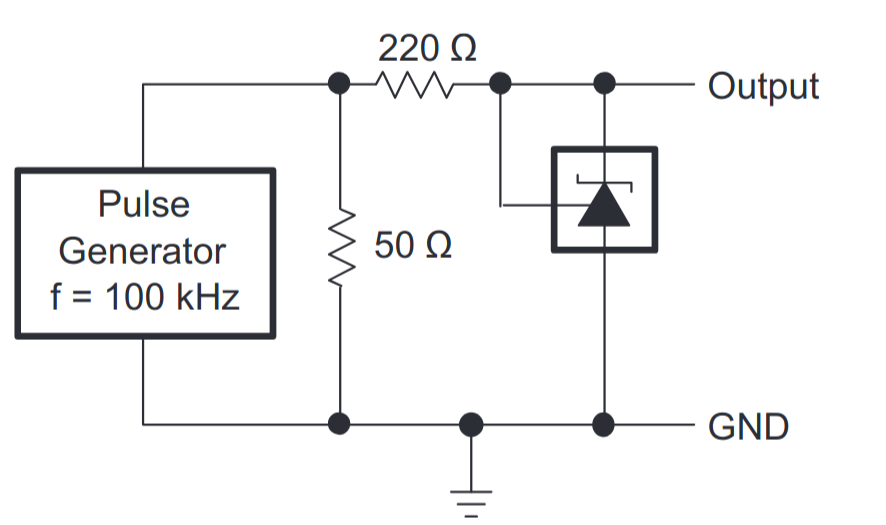
\includegraphics[width=0.5\linewidth]{Sablona_LaTeX/obrazky/TL431_pulse_cir.png}
            \caption{Zapojení s TL431 uvedené výrobcem pro testování pulzní odezvy \cite{TI_TL431_datasheet}}
            \label{fig:TL431_pulse_cir}
        \end{figure}
        

\clearpage
\newpage
\section{Závěr}
    V rámci této práce byly provedeny experimenty na~zapojení programovatelného proudového zdroje s~referenčním napětím. Základní funkcionalita zapojení spočívala v~generování stabilního proudu řízeného vnějším napětím. Hlavním cílem experimentů bylo ověřit funkčnost zapojení, analyzovat jeho vlastnosti a~zhodnotit jeho chování za~různých podmínek.
    \par
    Toto zapojení bylo poskytnuto vyučujícím (kapitola~\ref{sec:zadani}) a~jako klíčová součástka byla zvolena bočníková napěťová reference LT431 od~výrobce Texas~Instruments \cite{TI_TL431_datasheet} s~odpovídajícím modelem v~jazyce Spice \cite{TL431_spice_model}. Podrobnější rozbor součástky, jejího modelu i~zadaného zapojení je obsahem kapitol~\ref{sec:char_soucastky}, \ref{sec:rozhrani} a~\ref{sec:zapojeni}.
    \par
    Samotným experimentům se pak věnuje kapitola~\ref{sec:experimenty}, jež je rozdělena do~následujících podkapitol:
    \begin{enumerate}
        \item Experiment 1a (podkapitola \ref{subsec:1a}): simulace teplotní závislosti výstupního proudu a~srovnání s~údaji uvedenými výrobcem,
        \item Experiment 1b (podkapitola \ref{subsec:1b}): analýza maximální hodnoty zátěže v~závislosti na~parametrech zapojení (především napájecímu napětí), vyjádření analytického vztahu pro tuto závislost,
        \item Experiment 2 (podkapitola \ref{subsec:2}): šumová analýza výstupního proudu a~výkonu, srovnání s~šumovými charakteristikami poskytnutými výrobcem,
        \item Experiment 3 (podkapitola \ref{subsec:3}): srovnání simulované pulzní odezvy součástky TL431 s~tou poskytnutou výrobcem. 
    \end{enumerate}
    Podrobné závěry jednotlivých experimentů jsou obsahem vlastních podkapitol. 
    \par
    Obecně lze ale říci, že teplotní závislost simulovaného modelu je v~předpokládaných mezích. Maximální hodnota zatěžovacího odporu se~chová podle vztahu \ref{eq:Rmax}, což bylo experimentálně ověřeno. Šumová charakteristika zapojení není v~souladu s~popisem, jež uvádí výrobce~---~pravděpodobně v~důsledku nedokonalostí Spice modelu součástky. Srovnání pulzní odezvy obvodu vykazuje některé nesrovnalosti, které však mohou být přisouzeny vlastnostem zadaného zapojení.    

\clearpage
\newpage
\printbibliography

\newpage
\clearpage
\section{Přílohy}
\begin{lstlisting}[language=Python,label=ls:num_der,caption=Jednoduchý program pro numerickou derivaci dat z~experimentu~\ref{subsec:1a}]
import pandas as pd
import numpy as np

data = pd.read_csv('temp/1a_experiment.csv')

dx = np.gradient(data['temperature'])
dy = np.gradient(data['I(Rload)'])
derivative = dy / dx

# pridani derivace
data['dI_dT'] = derivative

# smazani sloupce
data = data.drop(columns=['I(Rload)'])

data.to_csv('temp/output.csv', index=False)
\end{lstlisting}

\begin{lstlisting}[label=ls:LT431,caption=Popis modelu klíčové součástky TL431 \cite{TL431_spice_model}]
*              REFERENCE
*              |  ANODE
*              |  |  CATHODE
*              |  |  |
.SUBCKT  TL431 1  2  3
V1  6  7  DC  1.4V
I1  2  4  1E-3
R1  1  2  1.2E6
R2  4  2  RMOD 2.495E3
R3  5  7  .2
D1  3  6  DMOD1
D2  2  3  DMOD1
D3  2  7  DMOD2
E1  5  2  POLY(2)  (4,2)  (1,2)  0  710  -710
.MODEL RMOD RES (TC1=1.4E-5 TC2=-1E-6)
.MODEL DMOD1 D (RS=.3)
.MODEL DMOD2 D (RS=1E-6)
.ENDS
\end{lstlisting}
\newpage
\clearpage
\begin{lstlisting}[label=ls:LT431,caption=Popis modelu bipolárního tranzistoru Q2N2222 poskytnutého vyučujícím]
.model Q2N2222	NPN(Is=14.34f Xti=3 Eg=1.11 Vaf=74.03 Bf=100 Ne=1.307
+		Ise=14.34f Ikf=.2847 Xtb=1.5 Br=6.092 Nc=2 Isc=0 Ikr=0 Rc=1
+		Cjc=38p Mjc=.3416 Vjc=.75 Fc=.5 Cje=126p Mje=.377 Vje=.75
+		Tr=200n Tf=12n Itf=.6 Vtf=1.7 Xtf=3 Rb=10)
\end{lstlisting}
\end{document}
